\chapter{Leading \Dijet \Xs{s}}
\label{chap:dijets}

%\chapterquote{Changing mass consciousness is an individual responsibility.}
%{Dennis Weaver}
%Mass demand has been created almost entirely through the development of advertising.
%{Calvin Coolidge}
\chapterquote{A short reign does not spare the masses.}
{Statius}

\section{Introduction}
As discussed in \ChapterRef{chap:forward-inclusive}, jet \xs measurements are an
important tool for probing theoretical predictions from \QCD. This analysis
examines the leading \dijet \xs as a function of the \dijet mass, \mDijet, in the region
$\yStar < 4.4$, where the variable \yStar is defined as half the rapidity difference
between the two leading (highest \pT) jets, $\yStar = |y_1 - y_2| / 2$, and is the
absolute rapidity of the \dijet{s} in their centre-of-mass frame. The results are
compared to expectations based on next-to-leading order (NLO) \QCD, corrected for
non-perturbative effects, as well as to NLO \MC predictions.

\section{\Xs Definition}
As for the inclusive jet \xs (\SectionRef{sec:forward-inclusive:cross_section_definition}),
the \dijet \xs is defined for the \ATLAS standard jet algorithms: \akt jets with
$R=0.4$ and $R =0.6$. The jet \xs measurements are, again, unfolded back to the
ideal particle level final state of the proton-proton collision. Identically to the
inclusive jet \xs, particle level jets in the \MC are identified with the same
jet algorithms as for data, using all stable particles and hence including muons
and neutrinos from decaying hadrons.

\section{Event Selection}
Similarly to the inclusive jets \xs, events are required to belong to a good run and
to have at least one good primary vertex (see \SectionRef{sec:analysis-tools:data_selection}).
The \dijet pair are selected as the two highest \pT jets in the event, provided
that these satisfy $\pT(j_1) \geq \unit{30}{\GeV}$, $\pT(j_2) \geq \unit{20}{\GeV}$ and
that both jets are within the acceptance region, $\absRap < 4.4$. If either of
these jets are flagged as ``bad'' or ``ugly'' by the standard medium jet
cleaning cuts, as detailed in \SectionRef{sec:analysis-tools:jet_cleaning}, then the event is
discarded. A pair of triggers appropriate to the transverse momentum and rapidity of the \dijet{s}
is then assigned - the event must pass one of these triggers in order to
contribute towards the \xs. Events passing this trigger selection are retained,
with a weight reflecting the amount of luminosity seen by the trigger
combination in question. Approximately 45\% of events passing these cuts contain
at least one additional jet which would also pass the cuts, however, the definition
used here, in which only the leading pair of jets is considered, ensures that there
is no ambiguity in such situations.

\section{Trigger Strategy}
\label{sec:dijets:trigger}
The trigger considerations for \dijet measurements are more complicated than for the
inclusive jet case because the \dijet \xs is measured as a function of the invariant
mass of the two-jet system and the rapidity separation \yStar, while jets are triggered
according to the jet transverse momentum. A per-event strategy based on invariant
mass, only considering events taken by triggers with $>99\%$ efficiency, would force
the use of highly prescaled low-threshold triggers to cover the mass ranges of interest.

The trigger strategy used for the inclusive jet \xs would be inefficient if directly transferred
to the \dijet case since only the two hardest jets in the event are important,
rather than all jets over a given \pT threshold. Similarly, a trigger strategy which
determined a single trigger that the event should pass, based on the \pT of the leading
jet in the event, would unnecessarily lose events due to the effects of prescale.

The strategy adopted is to define two possible trigger chains, based
on the \pT of the two leading jets, and to accept the event if either or both of
these are passed. A similar trigger strategy to that discussed in
\SectionRef{sec:forward-inclusive:trigger} is used: again dependent on the run
period and the \pT and \rap of the two leading jets. One important difference is that
whereas for the single jet \xs, triggers were selected based on whether the
\emph{per-event} efficiency was on plateau, here it must be required that the
\emph{per-jet} efficiency should be on plateau.

Using similar definitions to those discussed in \SectionRef{sec:forward-inclusive:trigger},
the rapidity interval in which jets can be accepted, $\absRap < 4.4$, is divided
into different regions: the central region, $\absRap < 2.9$; the transition region,
$2.9 \leq \absRap < 3.3$; the forward region $3.3 \leq \absRap < 3.6$ and the far-forward
region $3.6 \leq \absRap < 4.4$.

The trigger requirements are summarised in \TableRef{tab:dijets:central_triggers}
for central jets, \TableRef{tab:dijets:forward_triggers} for forward jets
and \TableRef{tab:dijets:far_forward_triggers} for far-forward jets. The transition
region presents additional complications which are discussed in \SectionRef{sec:dijets:transition_region_triggers}.

Having determined the two triggers that each event should pass, based on the \pT
of the two leading jets in the event, it is now required that one or both should have been passed
before the event can be accepted. All events which satisfy this condition are placed
into a trigger category defined by those specific two triggers, in other words,
one trigger category is created for each possible combination of the two triggers.

The equivalent luminosity seen by each trigger category can be calculated (see
\SectionRef{sec:dijets:effective_luminosity}) and the event can then be weighted
by the inverse of this effective luminosity before the final \xs measurements are
produced.

\begin{table}
\begin{center}
  \begin{tabular}{ l l l l l }
    \pT $[\GeV]$ & Run$<$152777 & Periods A--C & Periods D--F  &  Periods G--I       \\
                 &              &              & (minus E1--4) &                     \\
    \midrule
    20--42.5     & L1\_MBTS\_1  & L1\_MBTS\_1  & L1\_MBTS\_1   &  EF\_mbMbts\_1\_eff \\
    42.5--70     & L1\_MBTS\_1  & L1\_J5       & L1\_J5        &  EF\_j20\_jetNoEF   \\
    70--97.5     & L1\_MBTS\_1  & L1\_J15      & L1\_J15       &  EF\_j35\_jetNoEF   \\
    97.5--152.5  & L1\_MBTS\_1  & L1\_J30      & L1\_J30       &  EF\_j50\_jetNoEF   \\
    152.5--197.5 & L1\_MBTS\_1  & L1\_J55      & L1\_J55       &  EF\_j75\_jetNoEF   \\
    197.5--217.5 & L1\_MBTS\_1  & L1\_J55      & L1\_J55       &  EF\_j95\_jetNoEF   \\
    217.5+       & L1\_MBTS\_1  & L1\_J55      & L1\_J55       &  EF\_L1J95\_NoAlg   \\
  \end{tabular}
  \caption{The trigger chains used in the \dijet analysis for the central region, $\absRap<2.9$.}
  \label{tab:dijets:central_triggers}
\end{center}
\end{table}

\begin{table}
\begin{center}
  \begin{tabular}{ l l l l}
    \pT $[\GeV]$ & Periods A--C & Periods E--F  &  Periods G--I         \\
                 &              & (minus E1--4) &                      \\
    \midrule
    20--42.5     & L1\_MBTS\_1  & L1\_MBTS\_1   & EF\_mbMbts\_1\_eff   \\
    42.5--62.5   & L1\_MBTS\_1  & L1\_FJ10      & EF\_mbMbts\_1\_eff   \\
    62.5--72.5   & L1\_MBTS\_1  & L1\_FJ10      & EF\_fj30\_jetNoEF    \\
    72.5--95     & L1\_MBTS\_1  & L1\_FJ30      & EF\_fj30\_jetNoEF    \\
    95--160      & L1\_MBTS\_1  & L1\_FJ30      & EF\_fj50\_jetNoEF    \\
    160+         & L1\_MBTS\_1  & L1\_FJ30      & EF\_fj75\_jetNoEF    \\
  \end{tabular}
  \caption{The trigger chains used in the \dijet analysis for the forward region, $3.3\leq\absRap<3.6$.}
  \label{tab:dijets:forward_triggers}
\end{center}
\end{table}

\begin{table}
\begin{center}
  \begin{tabular}{ l l l l }
    \pT $[\GeV]$ & Periods A--E4 & Periods E5--F &  Periods G--I      \\
                 &               &               &                    \\
    \midrule
    20--42.5     & L1\_MBTS\_1   & L1\_FJ10      & EF\_mbMbts\_1\_eff \\
    42.5--50     & L1\_MBTS\_1   & L1\_FJ10      & EF\_fj30\_jetNoEF  \\
    50--67.5     & L1\_MBTS\_1   & L1\_FJ30      & EF\_fj30\_jetNoEF  \\
    67.5--100    & L1\_MBTS\_1   & L1\_FJ30      & EF\_fj50\_jetNoEF  \\
    100+         & L1\_MBTS\_1   & L1\_FJ30      & EF\_fj75\_jetNoEF  \\
  \end{tabular}
  \caption{The trigger chains used in the \dijet analysis for the far-forward region, $3.6\leq\absRap<4.4$.}
  \label{tab:dijets:far_forward_triggers}
\end{center}
\end{table}

\subsection{Trigger Complications in the Transition Region}
\label{sec:dijets:transition_region_triggers}
As discussed in \SectionRef{sec:forward-inclusive:transition_triggers}, there is
an ambiguity over whether to associate jets which are reconstructed in the transition
region, $2.9 \leq \absRap < 3.3$, with a central or a forward jet trigger. In this
region, which bridges the boundary between the central and forward calorimeters,
rapidity differences between L1 or L2 trigger jets
and offline jets can lead to central trigger jets that are reconstructed offline
as forward jets, and \emph{vice versa}. It can be seen in \FigureRef{fig:forward-inclusive:eta_efficiency_akt}
that the inefficiencies for central and forward triggers overlap by approximately 0.4
in rapidity.

Since each trigger is required to be on a per-jet efficiency plateau, different \pT bin boundaries are used in the central and forward
regions to optimise acceptance; it is, therefore, no longer enough to use a the simple central OR forward logic that could be applied to the
inclusive jet \xs. Accordingly, an angular ``matching'' is performed between offline
jets which fall into this region and trigger objects, to identify the closest trigger
jet and hence whether the offline jet should be classified as central or forward.

\subsubsection{Matching Offline Jets to L1 Triggers}
During periods A--F, when no HLT information was used for event selection,
offline jets must be matched to L1 trigger objects. However, \pseudorap
information is not retained by the FCAL at L1 and so simple \DeltaR matching cannot be
used without risking biases in trigger identification. First the closest \emph{forward} L1 trigger object is identified
as that with the smallest \DeltaPhi with respect to the offline jet. Next the closest
\emph{central} L1 trigger object is identified as that with the smallest \DeltaR
with respect to the offline jet; this takes advantage of the fact that \pseudorap information
is available for L1 objects in the central calorimeter. Having identified the
closest \emph{forward} and the closest \emph{central} L1 objects, whichever one
has the smaller \DeltaPhi separation with respect to the offline jet is assigned
as the best match.

\subsubsection{Matching Offline Jets to L2 Triggers}
In contrast to L1 objects, L2 trigger jets have \pseudorap information in all calorimeter
systems. For periods G--I therefore, when the HLT was in rejection mode, each offline
jet can be matched to the L2 trigger jet that is closest to it in \DeltaR; in other
words, the trigger jet that has the smallest \DeltaR with respect to the offline jet.
Since each L2 trigger jet is seeded by a L1 ROI, it can be uniquely determined whether
the L2 jet was seeded from a central or forward L1 ROI and hence whether the offline
jet should be associated with a central or forward trigger.

This procedure makes optimal use of such angular information as is available, avoiding
bias by using \DeltaPhi to discriminate among forward L1 ROIs, where \DeltaR would
tend to incorrectly assign forward jets as central. However it still takes advantage of
the \pseudorap information where possible in order to discriminate between central
L1 trigger jets.

\subsubsection{Determining \DeltaR and \DeltaPhi for Matching}
\label{sec:dijets:matching}
The matching procedures described above are subject to the constraint that an offline
jet is considered to be matched to a trigger jet only if they are separated by less
than a maximum value of $\DeltaR < 0.5$ or $\DeltaPhi < 0.4$, depending which metric
is used. The value of the maximum \DeltaR allowed for a match was chosen by inspecting
the \DeltaR distribution of the closest trigger jet, which is shown in
\FigureRef{fig:dijets:DeltaR}. The distribution has a Gaussian core that extends
to approximately $\DeltaR \simeq 0.5$. This Gaussian population indicates a genuine
correspondence between the offline jet and the closest trigger jet, where the smearing
arises from the fundamentally different way in which offline and trigger jets are constructed.
However, beyond this, in the region $\DeltaR > 0.5$, a large non-Gaussian tail dominates.
The non-Gaussian behaviour of this population indicates that these are mismatches,
and that the offline jet and its closest trigger jet in fact have no real association.
The boundary between these two populations occurring at $\DeltaR=0.5$ thus distinguishes
between real matches and mismatches, so it is the optimal value for the \DeltaR
matching cut.

A similar analysis was performed for the \DeltaPhi distribution shown
in \FigureRef{fig:dijets:DeltaPhi} in order to derive the optimal matching cut of
$\DeltaPhi < 0.4$. In both the \DeltaR and \DeltaPhi cases, the studies were performed
outside the region of interest, looking separately at more central jets, with $2.3 \leq \absRap < 2.9$
and more forward jets, with $3.3 \leq \absRap < 3.9$. This was done in order to
ensure that the choice of cut was not biased by inefficiencies in triggering that
would be present in the transition region. The distributions show a noticeable dependence
on the \pT region considered, with the lowest \pT region showing a large number of
events in which the best matched trigger jet is a large distance away from the offline
jet; this effect is an artefact of the low \pT offline jets considered
here. The low edge of the \pT bins used for this study is not yet on the efficiency plateau of the
relevant triggers, and so there will be cases in which a real offline jet has no
counterpart among the collection of trigger jets. In such cases, the closest matched
trigger jet will necessarily be an uncorrelated object which may therefore be a large
distance away. Since the jets used in the analysis are always on their trigger plateau
this is not an issue for the measurement. In fact the percentage of jets which are
rejected by this matching procedure as a result of the closest match being above the
cut is of the order of 0.5\%, depending on \pT, and a systematic error is assigned
to account for this.

\begin{figure}[htpb]
  \subfloat[L1 central jets]{
    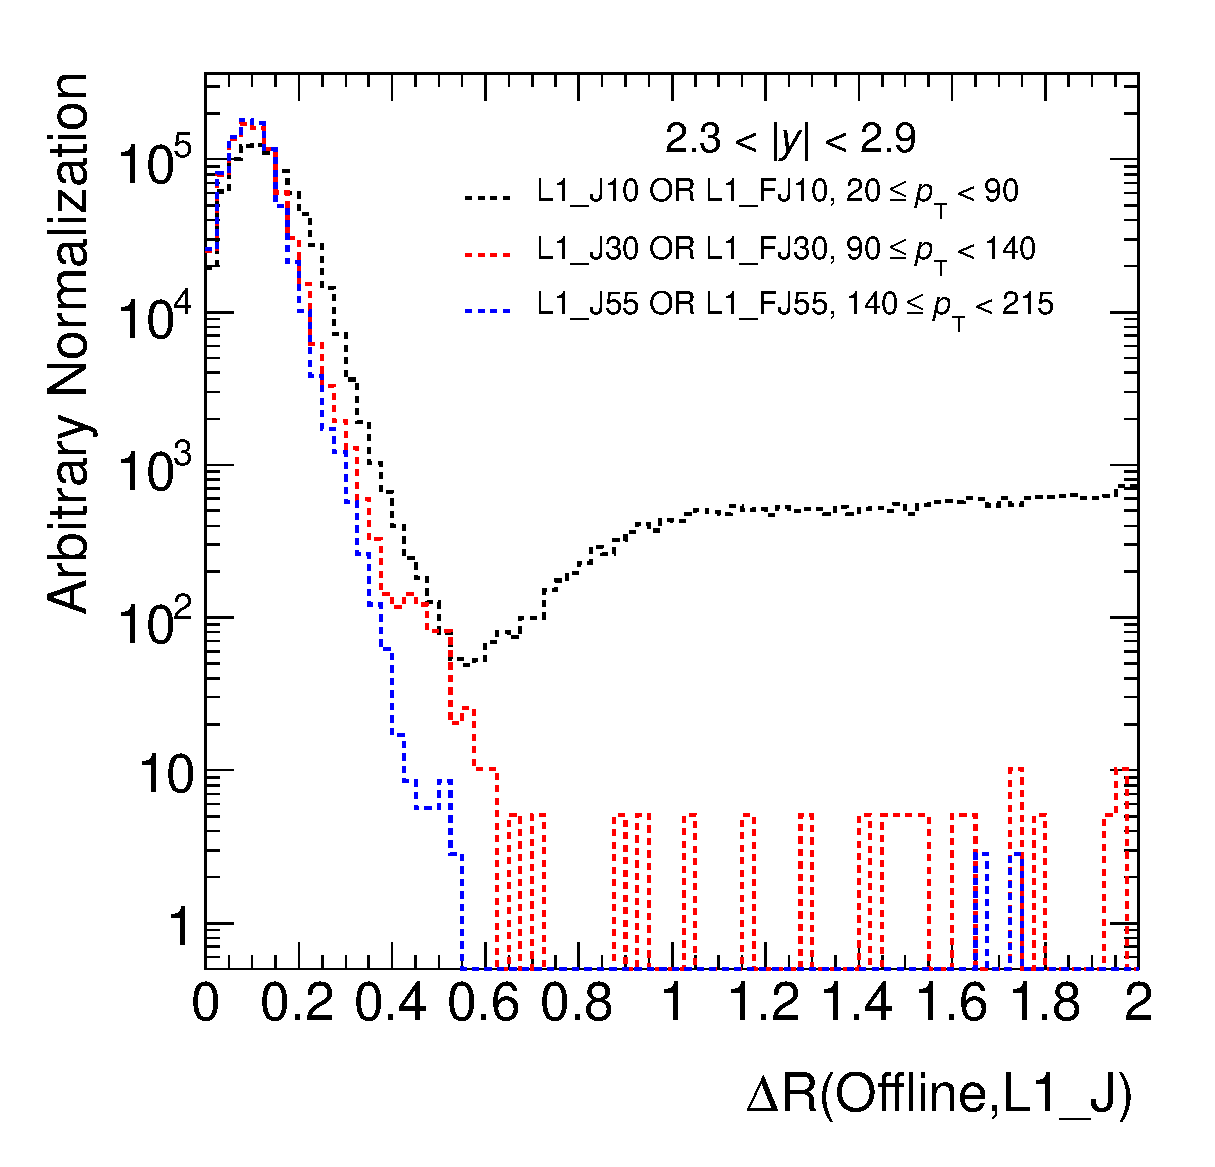
\includegraphics[width=\tinyfigwidth]{chapters/dijets/dR_L1j24_29.eps}
    \label{fig:dijets:dR_L1j24_29}}
  \quad
  \subfloat[L2 central jets]{
    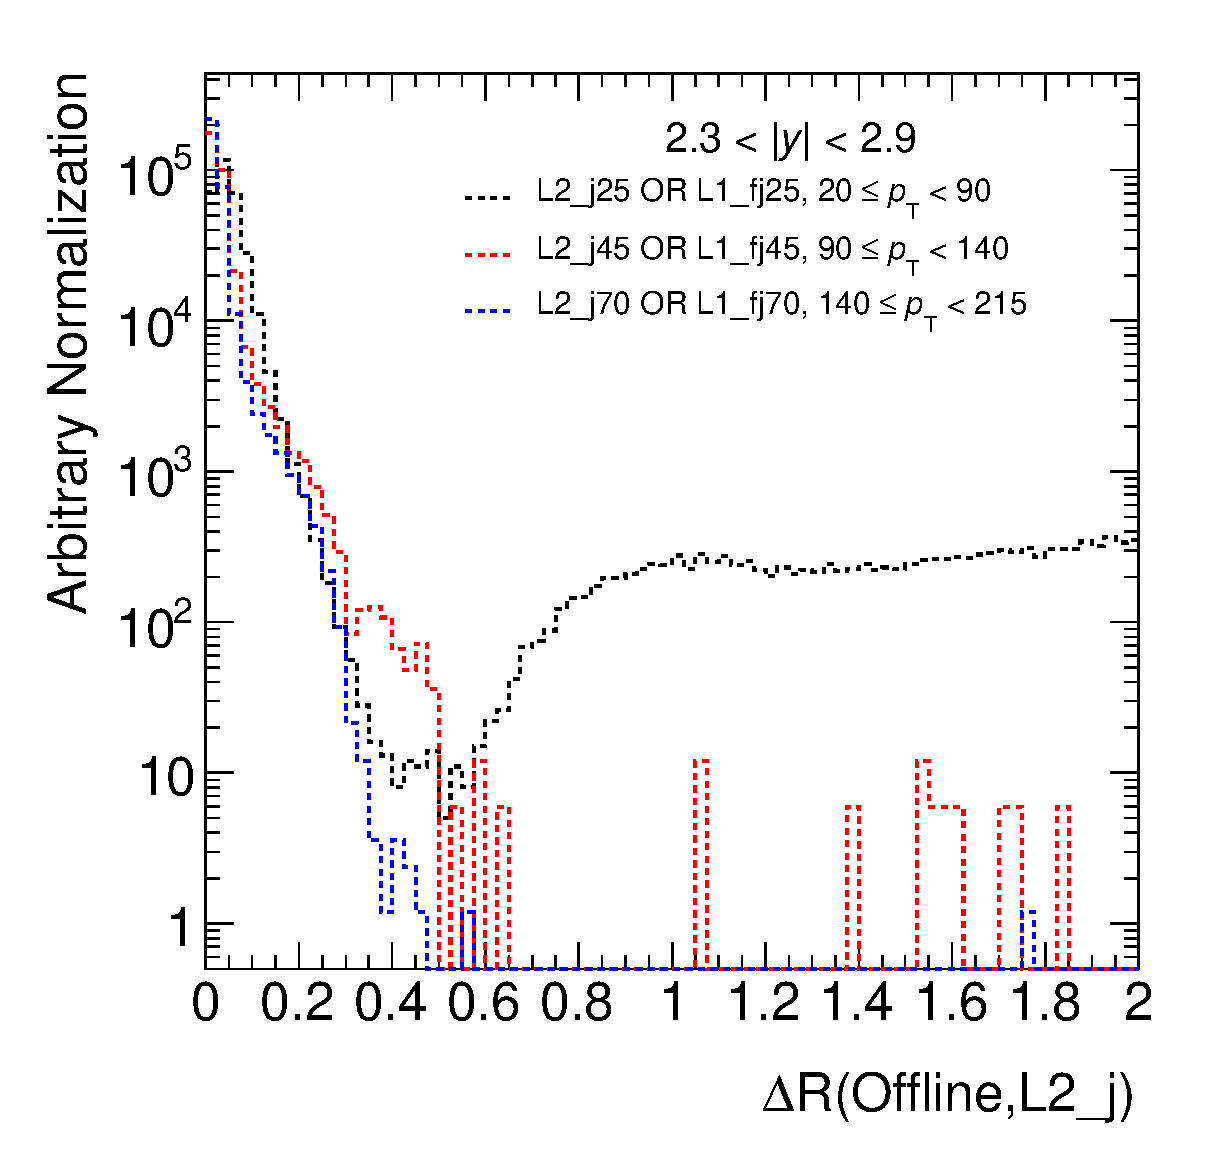
\includegraphics[width=\tinyfigwidth]{chapters/dijets/dR_L2j24_29.eps}
    \label{fig:dijets:dR_L2j24_29}}
  \quad
  \subfloat[L2 forward jets]{
    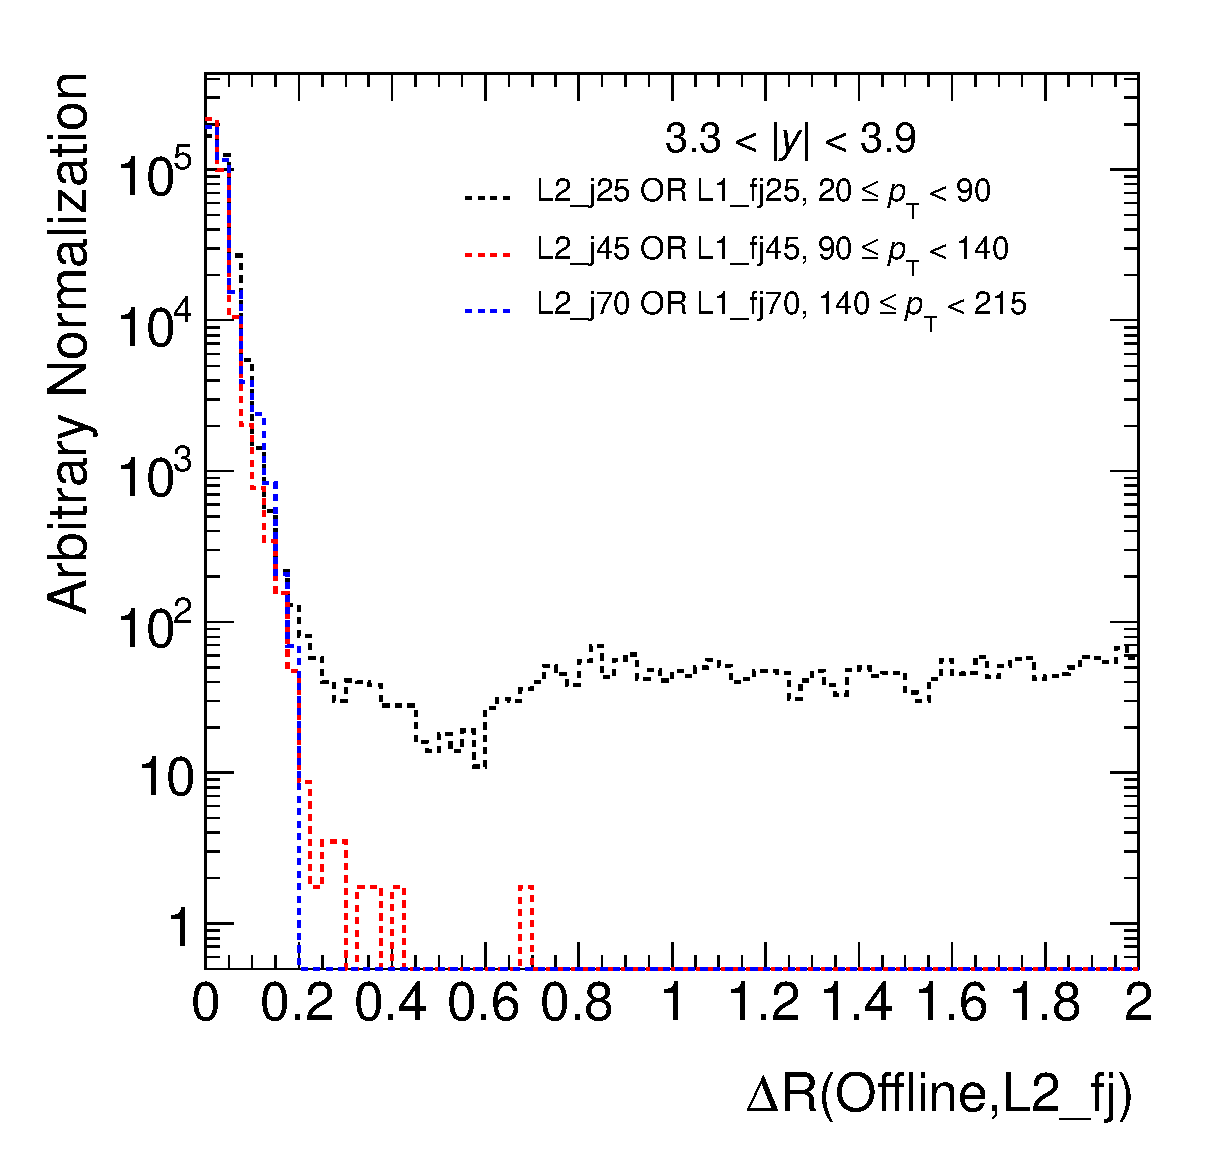
\includegraphics[width=\tinyfigwidth]{chapters/dijets/dR_L2fj34_39.eps}
    \label{fig:dijets:dR_L2fj34_39}}
  \caption{Angular separation \DeltaR between an offline jet and the closest trigger jet at L1 and L2. \protect\subref{fig:dijets:dR_L1j24_29} L1 central jets, \protect\subref{fig:dijets:dR_L2j24_29} L2 central jets and \protect\subref{fig:dijets:dR_L2fj34_39} are shown separately. The distribution is not shown for the forward region at L1 since the FCAL has no \pseudorap measurement at L1. The distributions indicate that the optimal \DeltaR cut to distinguish real matches from mismatches is $\DeltaR < 0.5$.}
  \label{fig:dijets:DeltaR}
\end{figure}

\begin{figure}[htpb]
  \subfloat[L1 central jets]{
    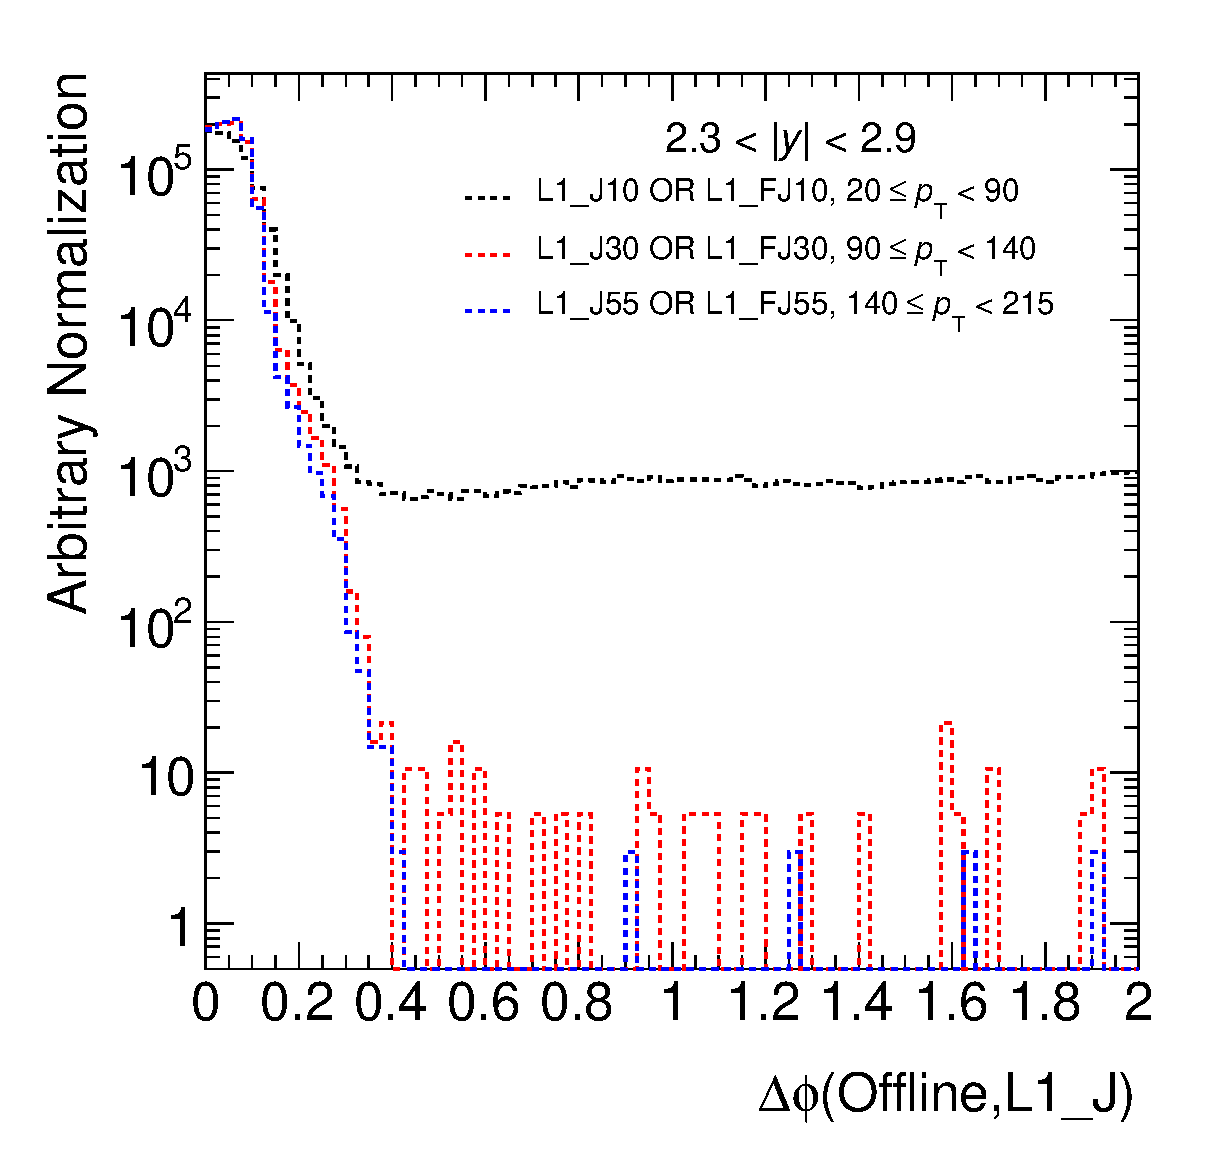
\includegraphics[width=\smallfigwidth]{chapters/dijets/dPhi_L1j24_29.eps}
    \label{fig:dijets:dPhi_L1j24_29}}
  \quad
  \subfloat[L1 forward jets]{
    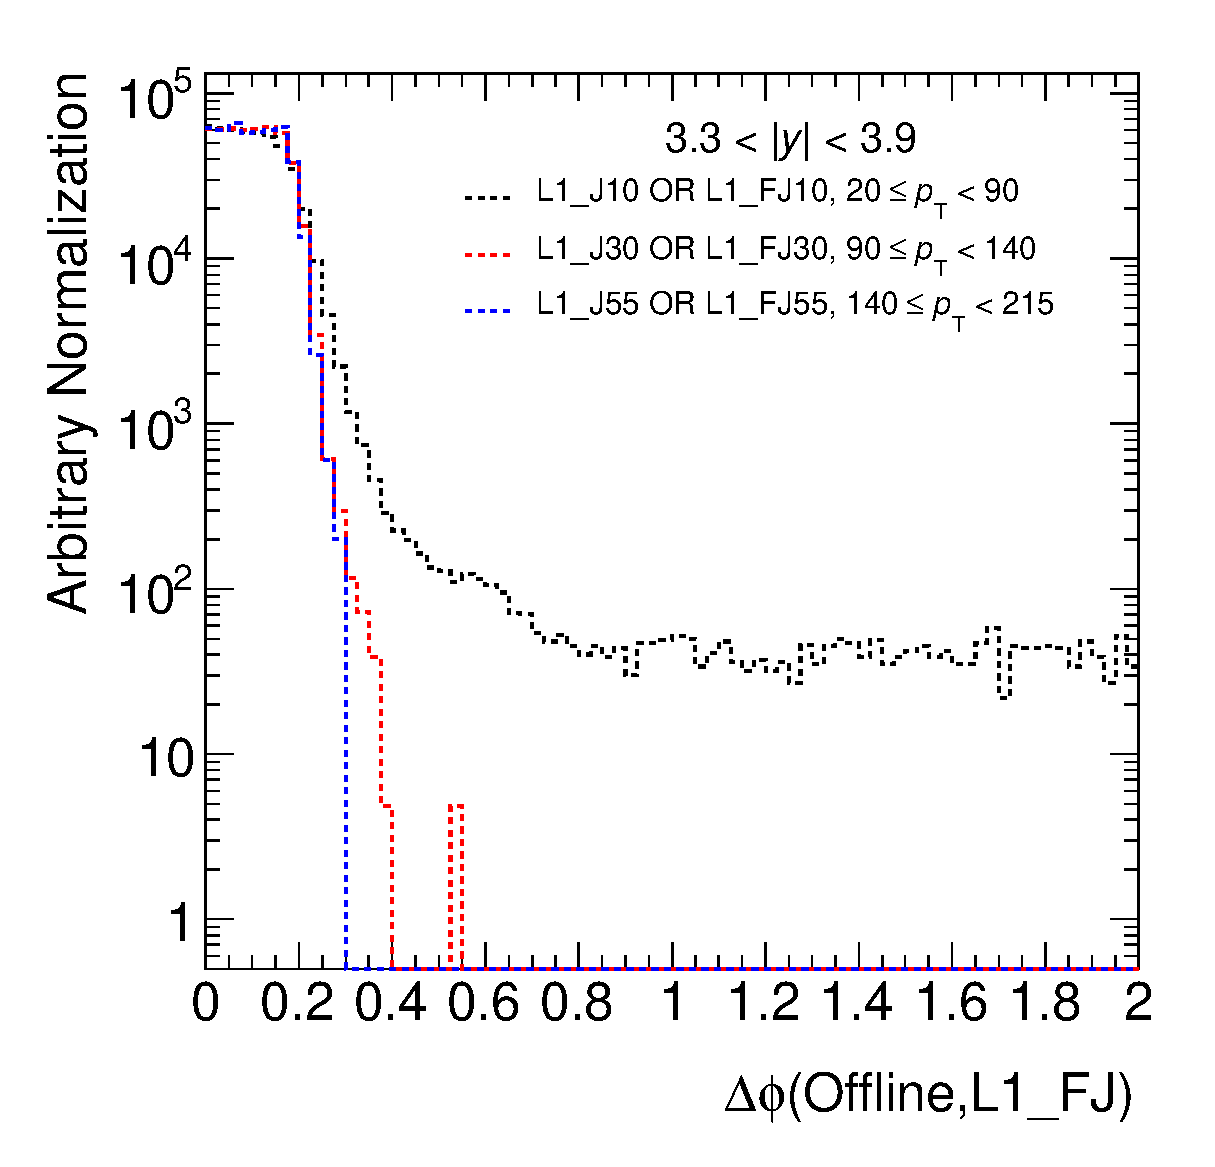
\includegraphics[width=\smallfigwidth]{chapters/dijets/dPhi_L1fj34_39.eps}
    \label{fig:dijets:dPhi_L1fj24_29}}
  \\
  \subfloat[L2 central jets]{
    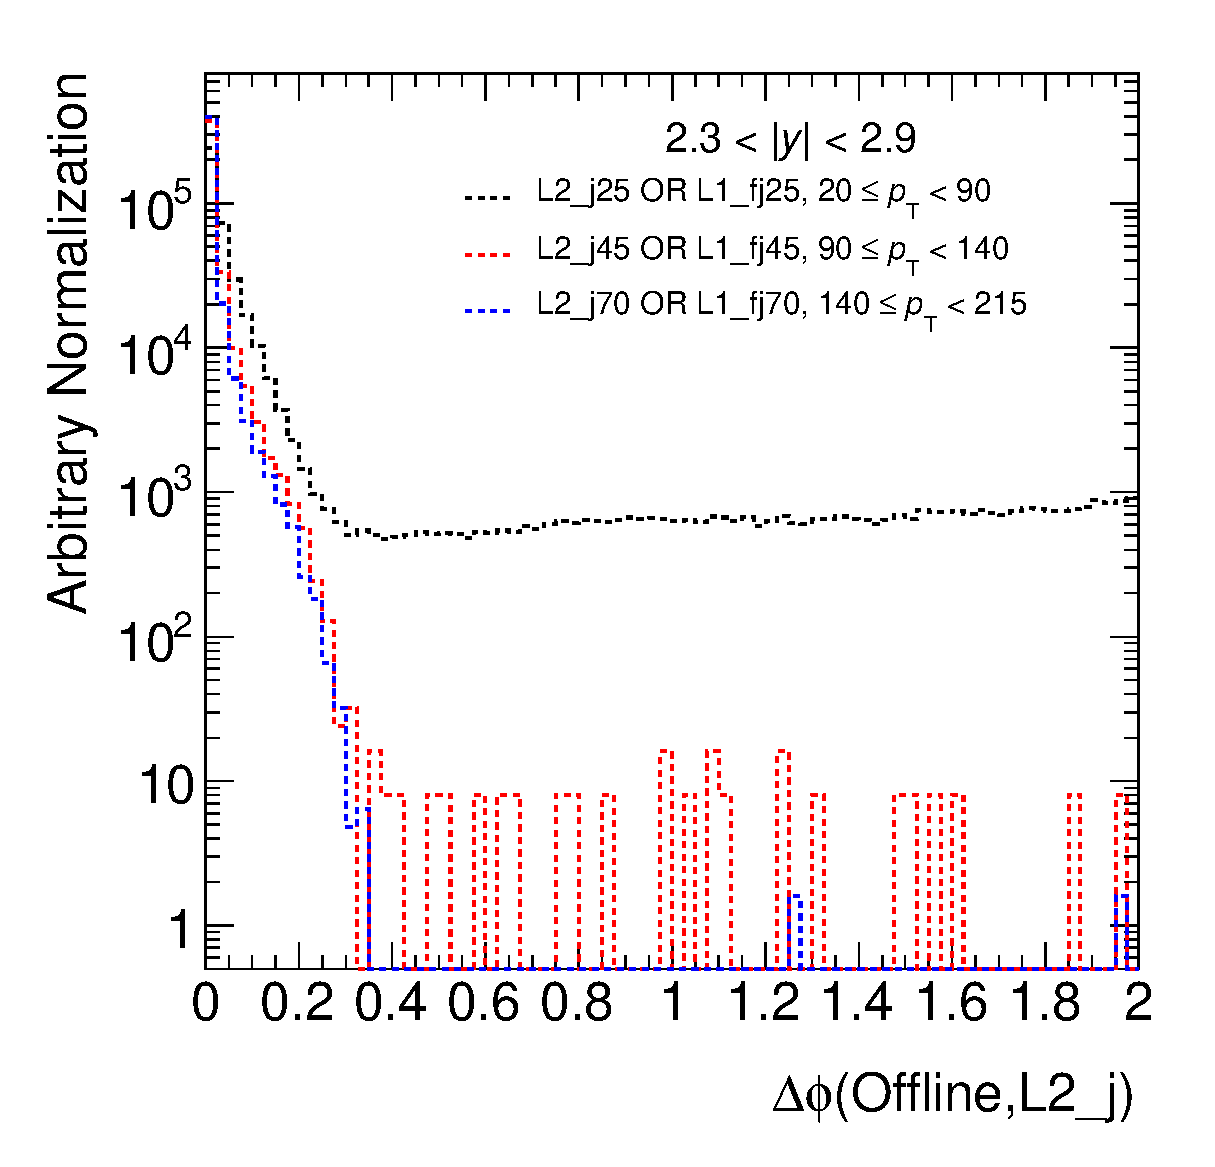
\includegraphics[width=\smallfigwidth]{chapters/dijets/dPhi_L2j24_29.eps}
    \label{fig:dijets:dPhi_L2j24_29}}
  \quad
  \subfloat[L2 forward jets]{
    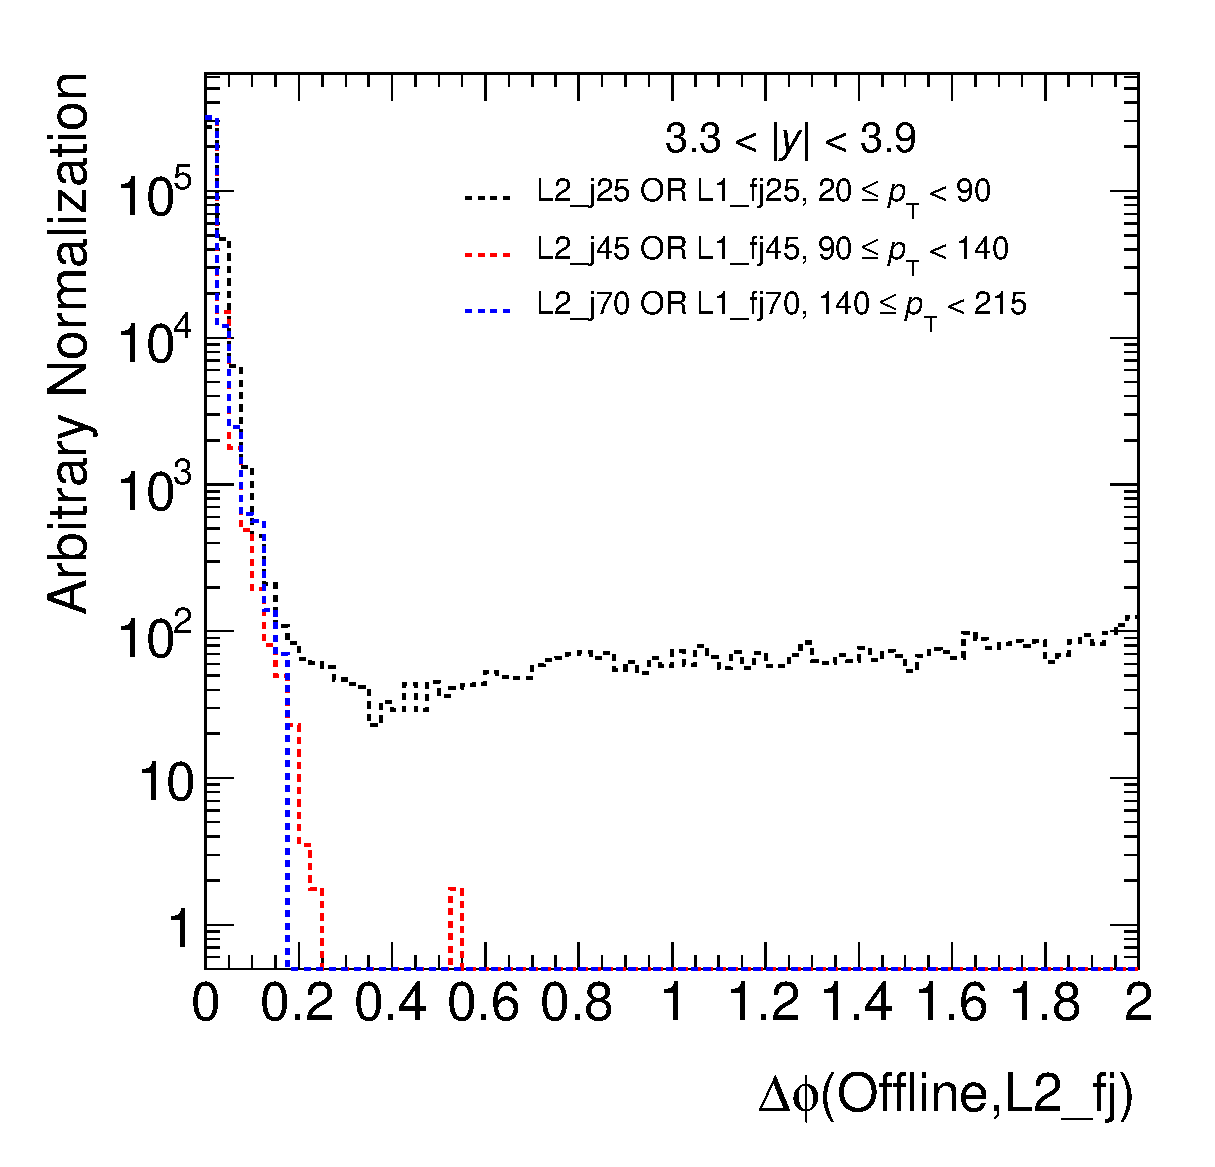
\includegraphics[width=\smallfigwidth]{chapters/dijets/dPhi_L2fj34_39.eps}
    \label{fig:dijets:dPhi_L2fj34_39}}
  \caption{Angular separation \DeltaPhi between an offline jet and the closest trigger
           jet at L1 (top) and L2 (bottom) for central jets (left) and forward jets
           (right). The distributions indicate that the optimal
           \DeltaPhi cut to distinguish real matches from mismatches is $\DeltaPhi < 0.4$.}
  \label{fig:dijets:DeltaPhi}
\end{figure}


\subsection{Per-Jet Trigger Inefficiencies}
Unlike the case of the inclusive jet efficiency, there is a ``crack'' region between
the calorimeter barrel and end-cap regions ($1.3 \leq \absRap \leq 1.6$) where the
per-jet trigger efficiency never becomes fully efficient due to calorimeter inhomogeneities.
The per-jet trigger efficiency in this crack region is shown in Table~\ref{tab:dijets:crack_efficiency}.

Additionally, due to a dead FCAL trigger tower that spans a width of $\Delta \phi=\pi/4$ in the
rapidity region $\eta>3.1$, the forward jet triggers are not fully efficient in
this region.  The per-jet efficiency is shown for the rapidity region $3.1 \leq \absRap < 3.6$
in \TableRef{tab:dijets:transition_efficiency} and for the forward region $3.6 \leq \absRap < 4.4$
in \TableRef{tab:dijets:forward_efficiency}.

A trigger efficiency correction is applied to any of the \dijet{s} that fall into either of these regions; in each case, the jet is weighted by the inverse of its trigger efficiency.
A systematic error is assigned for this procedure, equal to the maximal correction.

\begin{table}
\begin{center}
  \begin{tabular}{ l c c c }
    \pT $[\GeV]$ & Run$<152777$ & Run 152777--Period F & Period G--I \\
    \midrule
    20--42.5     & 1.00         & 1.00                 & 1.00       \\
    42.5--70     & 1.00         & 0.89                 & 0.96       \\
    70--97.5     & 1.00         & 0.88                 & 0.87       \\
    97.5--152.5  & 1.00         & 0.81                 & 0.83       \\
    152.5--197.5 & 1.00         & 0.83                 & 0.82       \\
    197.5--217.5 & 1.00         & 0.83                 & 0.80       \\
    217.5+       & 1.00         & 0.83                 & 0.81       \\
   \end{tabular}
  \caption{The plateau per-jet trigger efficiency in the crack region $1.3 \leq \absRap < 1.6$.
           Trigger inefficiency arises due to inhomogeneities in the crack region
           and is corrected for in the \dijet measurement.}
  \label{tab:dijets:crack_efficiency}
\end{center}
\end{table}

\begin{table}
\begin{center}
  \begin{tabular}{ l c c c }
    \pT $[\GeV]$ & Periods A--D & Periods E--F  & Period G--I \\
                 &              & (minus E1--4) &              \\
    \midrule
    20--42.5     & 1.00         & 1.00          & 1.00       \\
    42.5--62.5   & 1.00         & 1.00          & 1.00       \\
    62.5--72.5   & 1.00         & 1.00          & 0.99       \\
    72.5--95     & 1.00         & 0.97          & 0.99       \\
    95--160      & 1.00         & 0.97          & 0.99       \\
    160+         & 1.00         & 0.97          & 1.00       \\
   \end{tabular}
  \caption{The per-jet trigger efficiency for the jet rapidity region $3.1 \leq \absRap < 3.6$.
           Trigger inefficiency arises due to the dead FCAL tower and is corrected
           for in the \dijet measurement.}
  \label{tab:dijets:transition_efficiency}
\end{center}
\end{table}

\begin{table}
\begin{center}
  \begin{tabular}{ l c c c }
    \pT $[\GeV]$ & Periods A--D & Periods E--F  & Period G--I \\
                 &              & (minus E1--4) &             \\
    \midrule
    20--42.5     & 1.00         & 0.95          & 1.00        \\
    42.5--50     & 1.00         & 0.95          & 0.99        \\
    50--67.5     & 1.00         & 0.95          & 0.99        \\
    67.5--100    & 1.00         & 0.95          & 0.97        \\
    100+         & 1.00         & 0.95          & 0.97        \\
   \end{tabular}
  \caption{The per-jet trigger efficiency for the jet rapidity region $3.6 \leq \absRap < 4.4$.
           Trigger inefficiency arises due to the dead FCAL tower and is corrected
           for in the \dijet measurement.}
  \label{tab:dijets:forward_efficiency}
\end{center}
\end{table}

\subsection{Calculating Effective Luminosity}
\label{sec:dijets:effective_luminosity}
In \SectionRef{sec:forward-inclusive:transition_triggers} it was possible to determine
a \xs for the case in which multiple triggers were used by dividing events up according
to which triggers they would have passed before prescale. Here, however, the number
of trigger categories is large and hence it would be preferable not to divide up the number
of events any further.

Given that the triggers are selected in such a way that they are on plateau in the
relevant region, it is expected that, in the absence of efficiency or prescale
effects, all events should pass both of the appropriate triggers. Defining the case where the leading
jet passes its trigger as $T_{10}$ and the case where the second jet passes its trigger
as $T_{01}$, this would mean that all events belong to case $T_{11}$.

In the hypothetical case where the leading and second jet triggers had respective
prescales $P^{\mathrm{L}}$ and $P^{\mathrm{S}}$ but no inefficiencies, some events would
move to $T_{10}$, some to $T_{01}$ and some to $T_{00}$. The effective luminosity
for the events remaining in one of $T_{10}$, $T_{01}$ and $T_{11}$ would be,
after summing over all luminosity blocks, LB:

\begin{equation}
  \mathcal{L}_{\mathrm{effective}} = \sum_{\mathrm{LB}} \frac{\mathcal{L}_{\mathrm{LB}}}{P^{\mathrm{L}}_{\mathrm{LB}} P^{\mathrm{S}}_{\mathrm{LB}}/(P^{\mathrm{L}}_{\mathrm{LB}} + P^{\mathrm{S}}_{\mathrm{LB}}-1)}
\end{equation}

\noindent where $\mathcal{L}_{\mathrm{LB}}$ is the luminosity of each luminosity block.
This is simply the degenerate case of \EquationRef{eq:forward-inclusive:final_luminosity}
in which all events belong to the last category. Unlike that situation, however,
it is no longer important which events belong to which category before prescale: an
identical effective luminosity can be applied to all events in the trigger category.

With the addition of trigger inefficiencies, the situation becomes slightly more
complicated. However, after compensating for inefficiency, only the total number
of events needs to be determined. It can be demonstrated, see \AppendixRef{chap:appendix:trigger_efficiencies},
that, if events are weighted as shown in \TableRef{tab:dijets:efficiency_correction}, then this total
number of events can be correctly recovered: although the individual
numbers no longer directly indicate which triggers were passed, the total number
passing one of the two triggers is correct.

\begin{table}
\begin{center}
  \begin{tabular}{ l l }
    Triggers passed (after prescale) & Efficiency weighting          \\
    \midrule
    Leading jet ($T_{10}$)           & $1/e_L$                       \\
    Second jet ($T_{01}$)            & $1/e_S$                       \\
    Both triggers ($T_{11}$)         & $1/e_L + 1/e_S - 1/(e_L*e_S)$ \\
   \end{tabular}
  \caption{The efficiency weightings for different combinations of passed triggers.
           $e_L$ is the efficiency of the leading jet trigger and $e_S$ is the efficiency
           of the second jet trigger.}
  \label{tab:dijets:efficiency_correction}
\end{center}
\end{table}

\section{Validating the Two-Trigger Strategy}
This trigger procedure was validated to ensure that it gave compatible results with
a simpler single-trigger strategy. Additionally, investigations were made to determine
optimum values for the matching cuts, which are discussed in \SectionRef{sec:dijets:matching}.
Finally a closure test was performed with \MC, where the effects of the trigger
have been emulated using the prescale values of a typical run.

The implementation of this method is validated using a closure test with Monte
Carlo, where the effects of the trigger are emulated using the prescale values
of a typical run. \MC events are discarded at random according to the prescales
of the triggers appropriate to the \dijet pair, with the surviving events constituting
a ``triggered pseudodata'' sample, which is then analysed with the same procedure as is used
for data. In particular, the pseudo-triggered events are assigned to trigger categories, the
\dijet mass histogram from each trigger category is divided by the appropriate
equivalent luminosity, and finally the resulting \xs{s} from all the trigger categories
are combined to obtain the final detector level results.

The resulting \dijet mass spectrum in slices of the rapidity separation \yStar from
0.0 to 4.4 is shown in \FigureRef{fig:dijets:closure} for both the pseudo-triggered and untriggered
\MC samples. The distributions obtained after trigger emulation and correction using the trigger
analysis code are compatible, within the available statistics, with the same distributions from the original
\MC sample without the trigger requirement, hence validating the two-jet trigger method.

\begin{figure}[htpb]
  \subfloat[\Dijet closure $0.0 \leq \yStar < 4.4$]{
    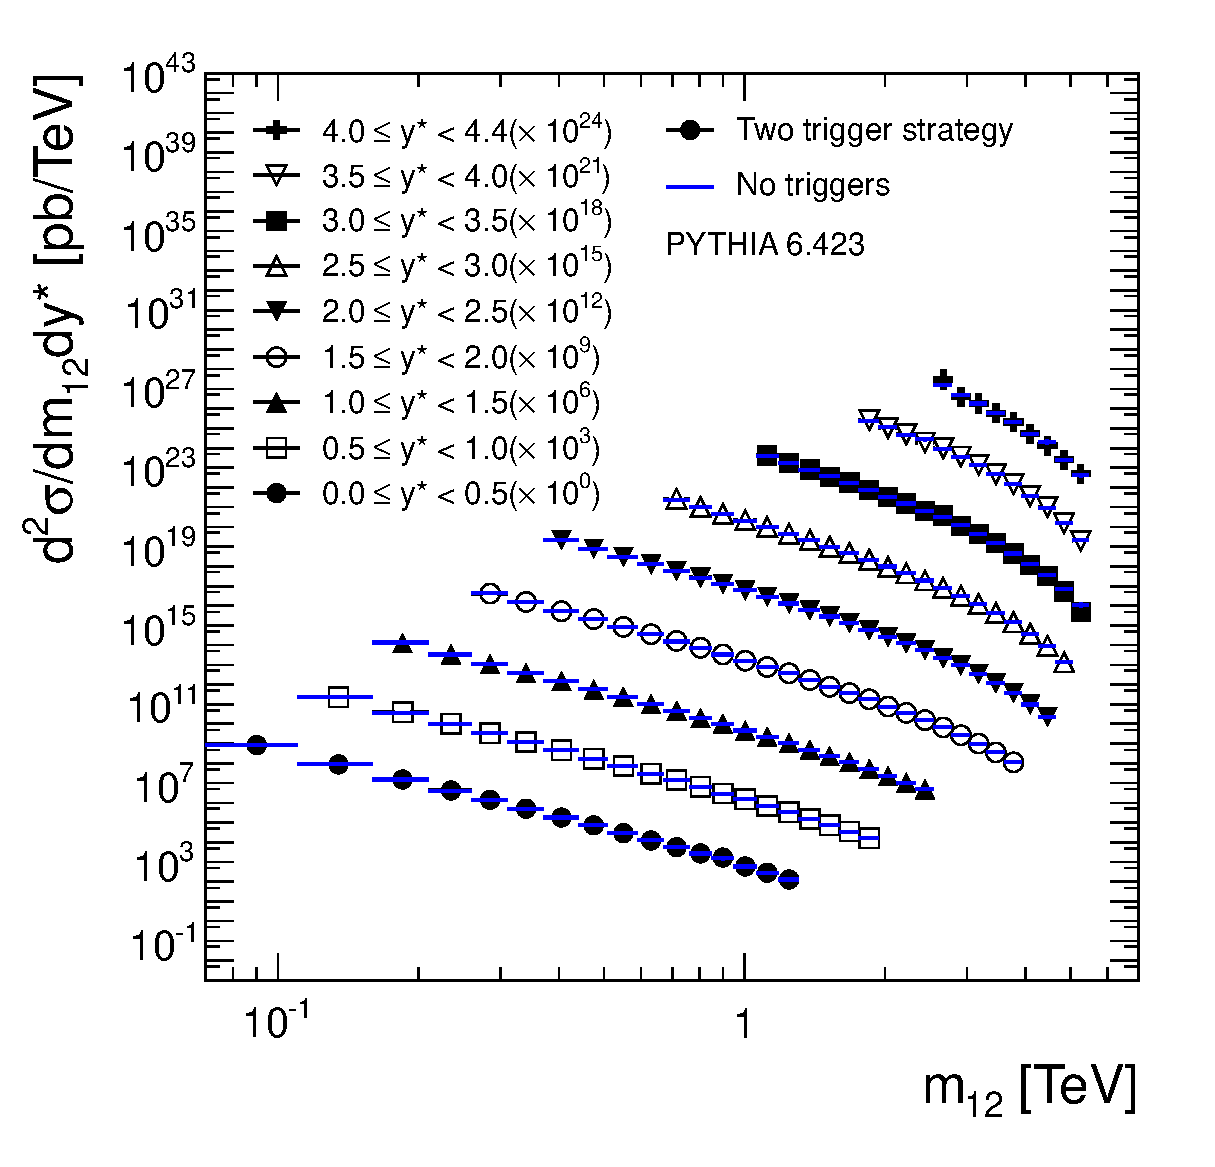
\includegraphics[width=\smallfigwidth]{chapters/dijets/DijetClosure.AntiKt6.yStar.eps}
    \label{fig:dijets:closure_all}}
  \quad
  \subfloat[\Dijet closure, $1.0 \leq \yStar < 1.5$]{
    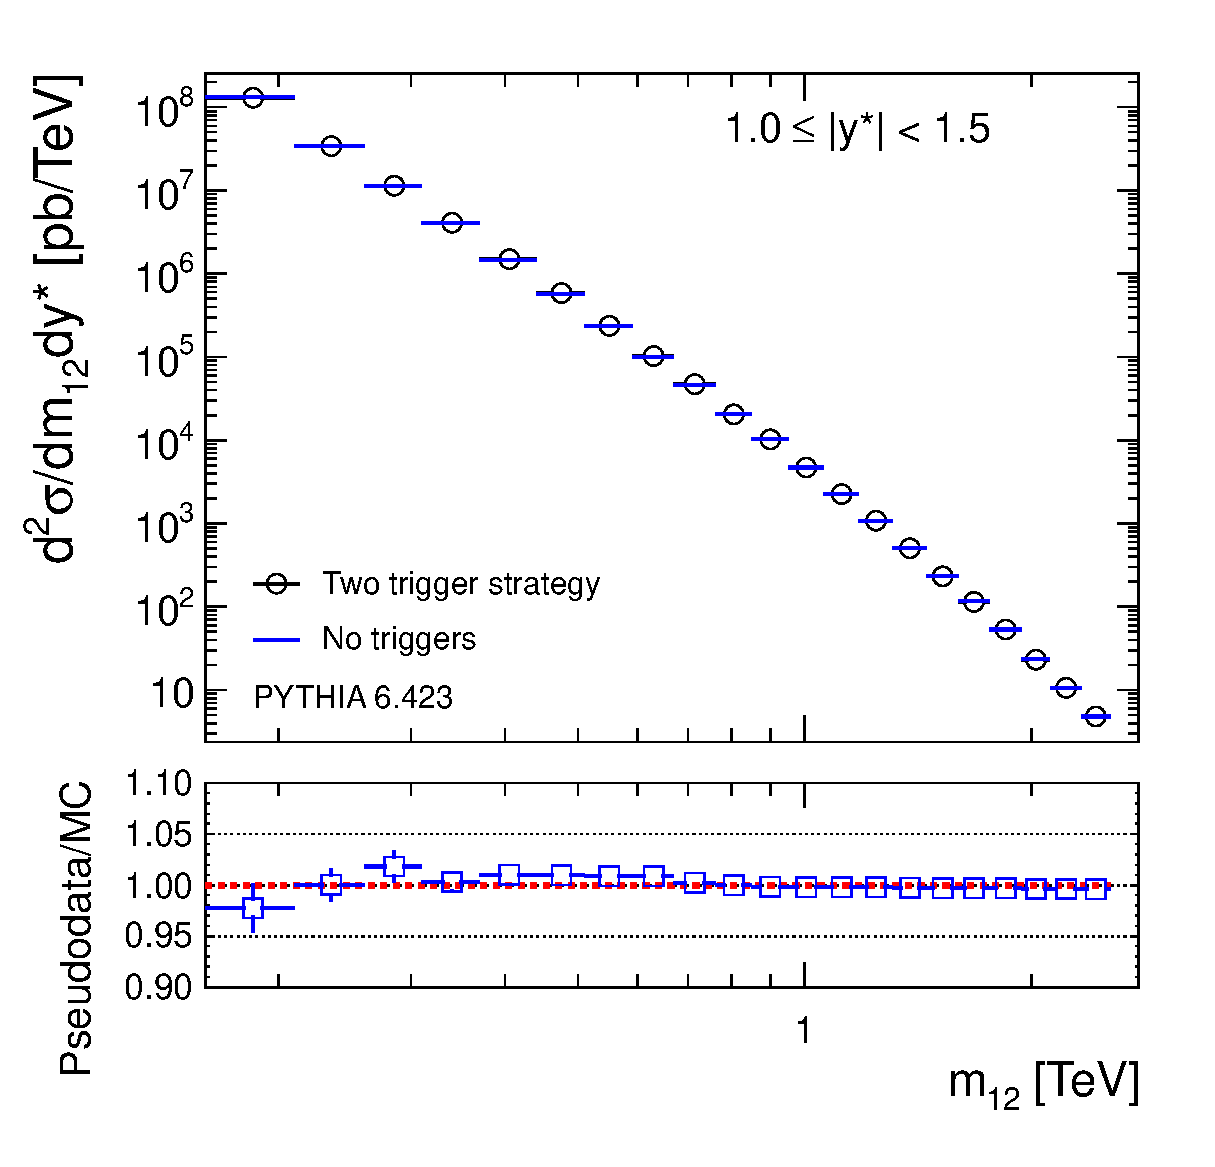
\includegraphics[width=\smallfigwidth]{chapters/dijets/DijetClosure.AntiKt6.yStar1.0_1.5.eps} %DijetClosure.AntiKt6.yStar1.5_2.0.eps}
    \label{fig:dijets:closure_ratio}}
  \caption{Summary of the closure test for a \dijet \MC sample for jets identified using the \akt algorithm with $R=0.6$. The black dots represent the result of emulating the trigger in the \MC and then correcting for it using the same technique used on data (the pseudodata sample), while the blue solid lines (overlaid) represent the result of analysing all events, without trigger corrections (the \MC sample). The results are presented in \protect\subref{fig:dijets:closure_all} as a function of \mDijet in different \yStar bins while in \protect\subref{fig:dijets:closure_ratio} the case $1.0 \leq \yStar < 1.5$ is shown separately, together with the ratio of pseudodata to \MC in each mass bin.}
  \label{fig:dijets:closure}
\end{figure}

\section{Effective Luminosities}
For the \dijet measurements, the luminosities are calculated for the two-jet trigger
scheme used (see \TableRangeRef{tab:dijets:central_triggers}{tab:dijets:far_forward_triggers}).
The effective luminosities for different trigger combinations
are shown for Periods A--D in \TableRef{tab:dijets:LumiDijetPeriodAD}, for Periods E5--F
in \TableRef{tab:dijets:LumiDijetPeriodE5F}, and for Periods G--I in \TableRef{tab:dijets:LumiDijetPeriodGI}.

\begin{table}
\begin{center}
  \begin{tabular}{ r r@{.}l r@{.}l r@{.}l r@{.}l r@{.}l }
                & \multicolumn{2}{l}{L1\_MBTS\_1} & \multicolumn{2}{l}{L1\_J5}  & \multicolumn{2}{l}{L1\_J15} & \multicolumn{2}{l}{L1\_J30} & \multicolumn{2}{l}{L1\_J55} \\
    \cmidrule{2-11}
    L1\_MBTS\_1 & 0&0005827                       & 0&02627                     & 0&2723                      & 0&2723                      & 0&2723                      \\
    L1\_J5      & \multicolumn{2}{l}{}            & 0&2723                      & 0&2723                      & 0&2723                      & 0&2723                      \\
    L1\_J15     & \multicolumn{2}{l}{}            & \multicolumn{2}{l}{}        & 0&2723                      & 0&2723                      & 0&2723                      \\
    L1\_J30     & \multicolumn{2}{l}{}            & \multicolumn{2}{l}{}        & \multicolumn{2}{l}{}        & 0&2723                      & 0&2723                      \\
    L1\_J55     & \multicolumn{2}{l}{}            & \multicolumn{2}{l}{}        & \multicolumn{2}{l}{}        & \multicolumn{2}{l}{}        & 0&2723                      \\
  \end{tabular}
  \caption{Effective luminosity in \ipb of different trigger combinations used in
           Periods A--D.}
  \label{tab:dijets:LumiDijetPeriodAD}
\end{center}
\end{table}

\begin{table}
\begin{center}
  \begin{tabular}{ r r@{.}l r@{.}l r@{.}l r@{.}l }
                & \multicolumn{2}{l}{L1\_MBTS\_1} & \multicolumn{2}{l}{L1\_J5}   & \multicolumn{2}{l}{L1\_J15}  & \multicolumn{2}{l}{L1\_J30} \\
    \cmidrule{2-9}
    L1\_MBTS\_1 & 0&00008220                      & 0&002549                     & 0&02488                      & 1&136                       \\
    L1\_J5      & \multicolumn{2}{l}{}            & 0&002473                     & 0&02728                      & 1&137                       \\
    L1\_J15     & \multicolumn{2}{l}{}            & \multicolumn{2}{l}{}         & 0&02489                      & 1&140                       \\
    L1\_J30     & \multicolumn{2}{l}{}            & \multicolumn{2}{l}{}         & \multicolumn{2}{l}{}         & 1&136                       \\
                & \multicolumn{2}{l}{L1\_J55}     & \multicolumn{2}{l}{L1\_FJ10} & \multicolumn{2}{l}{L1\_FJ30} & \multicolumn{2}{l}{}        \\
    \cmidrule{2-9}
    L1\_MBTS\_1 & 2&251                           & 0&01606                      & 2&251                        & \multicolumn{2}{l}{}        \\
    L1\_J5      & 2&251                           & 0&01844                      & 2&251                        & \multicolumn{2}{l}{}        \\
    L1\_J15     & 2&251                           & 0&04019                      & 2&251                        & \multicolumn{2}{l}{}        \\
    L1\_J30     & 2&251                           & 1&137                        & 2&251                        & \multicolumn{2}{l}{}        \\
    L1\_J55     & 2&251                           & 2&251                        & 2&251                        & \multicolumn{2}{l}{}        \\
    L1\_FJ10    & \multicolumn{2}{l}{}            & 0&01600                      & 2&251                        & \multicolumn{2}{l}{}        \\
    L1\_FJ30    & \multicolumn{2}{l}{}            & \multicolumn{2}{l}{}         & 2&251                        & \multicolumn{2}{l}{}        \\
  \end{tabular}
  \caption{Effective luminosity in \ipb of different trigger combinations used in
           Periods E5--F.}
  \label{tab:dijets:LumiDijetPeriodE5F}
\end{center}
\end{table}

\begin{table}
\begin{center}
  \begin{tabular}{ r r@{.}l r@{.}l r@{.}l r@{.}l }
                   & \multicolumn{2}{l}{mbMbts\_1\_eff} & \multicolumn{2}{l}{j20\_jetNoEF}  & \multicolumn{2}{l}{j35\_jetNoEF}  & \multicolumn{2}{l}{j50\_jetNoEF}  \\
    \cmidrule{2-9}
    mbMbts\_1\_eff & 0&0001021                          & 0&002504                          & 0&05213                           & 0&2541                            \\
    j20\_jetNoEF   & \multicolumn{2}{l}{}               & 0&002418                          & 0&05437                           & 0&2578                            \\
    j35\_jetNoEF   & \multicolumn{2}{l}{}               & \multicolumn{2}{l}{}              & 0&05203                           & 0&2782                            \\
    j50\_jetNoEF   & \multicolumn{2}{l}{}               & \multicolumn{2}{l}{}              & \multicolumn{2}{l}{}              & 0&2556                            \\
                   & \multicolumn{2}{l}{j75\_jetNoEF}   & \multicolumn{2}{l}{fj30\_jetNoEF} & \multicolumn{2}{l}{fj50\_jetNoEF} & \multicolumn{2}{l}{fj75\_jetNoEF} \\
    \cmidrule{2-9}
    mbMbts\_1\_eff & 6&507                              & 0&1643                            & 3&871                             & 35&69                             \\
    j20\_jetNoEF   & 6&508                              & 0&1665                            & 3&873                             & 35&69                             \\
    j35\_jetNoEF   & 6&521                              & 0&1891                            & 3&889                             & 35&69                             \\
    j50\_jetNoEF   & 6&569                              & 0&3424                            & 3&951                             & 35&69                             \\
    j75\_jetNoEF   & 6&507                              & 6&558                             & 7&906                             & 35&69                             \\
    fj30\_jetNoEF  & \multicolumn{2}{l}{}               & 0&1642                            & 3&937                             & 35&69                             \\
    fj50\_jetNoEF  & \multicolumn{2}{l}{}               & \multicolumn{2}{l}{}              & 3&871                             & 35&69                             \\
    fj75\_jetNoEF  & \multicolumn{2}{l}{}               & \multicolumn{2}{l}{}              & \multicolumn{2}{l}{}              & 35&69                             \\
  \end{tabular}
  \caption{Effective luminosity in \ipb of different trigger combinations used in
           Periods G--I. The initial ``EF\_'' has been left off all trigger names
           for brevity.}
  \label{tab:dijets:LumiDijetPeriodGI}
\end{center}
\end{table}

\section{Unfolding Detector Effects}
Unfolding of the \dijet \xs{s} is performed using the IDS method as described
in \SectionRef{sec:forward-inclusive:unfolding}. The same binning is used as for
the final distributions and the particle level spectra in \MC are reweighted to
correct for any shape mismodelling as discussed previously.

\FigureRef{fig:dijets:data_mc_control_distributions} shows the level of agreement
between \Pythia and the data for two sample distributions; an event-by-event reweighting
function is calculated and applied to the particle level spectra in \MC to eliminate
any effects of shape differences between data and \MC.

\begin{figure}[htpb]
  \subfloat[Data to \MC comparison for \akt $R=0.4$, in the region $0.5 \leq \yStar < 1.0$]{
    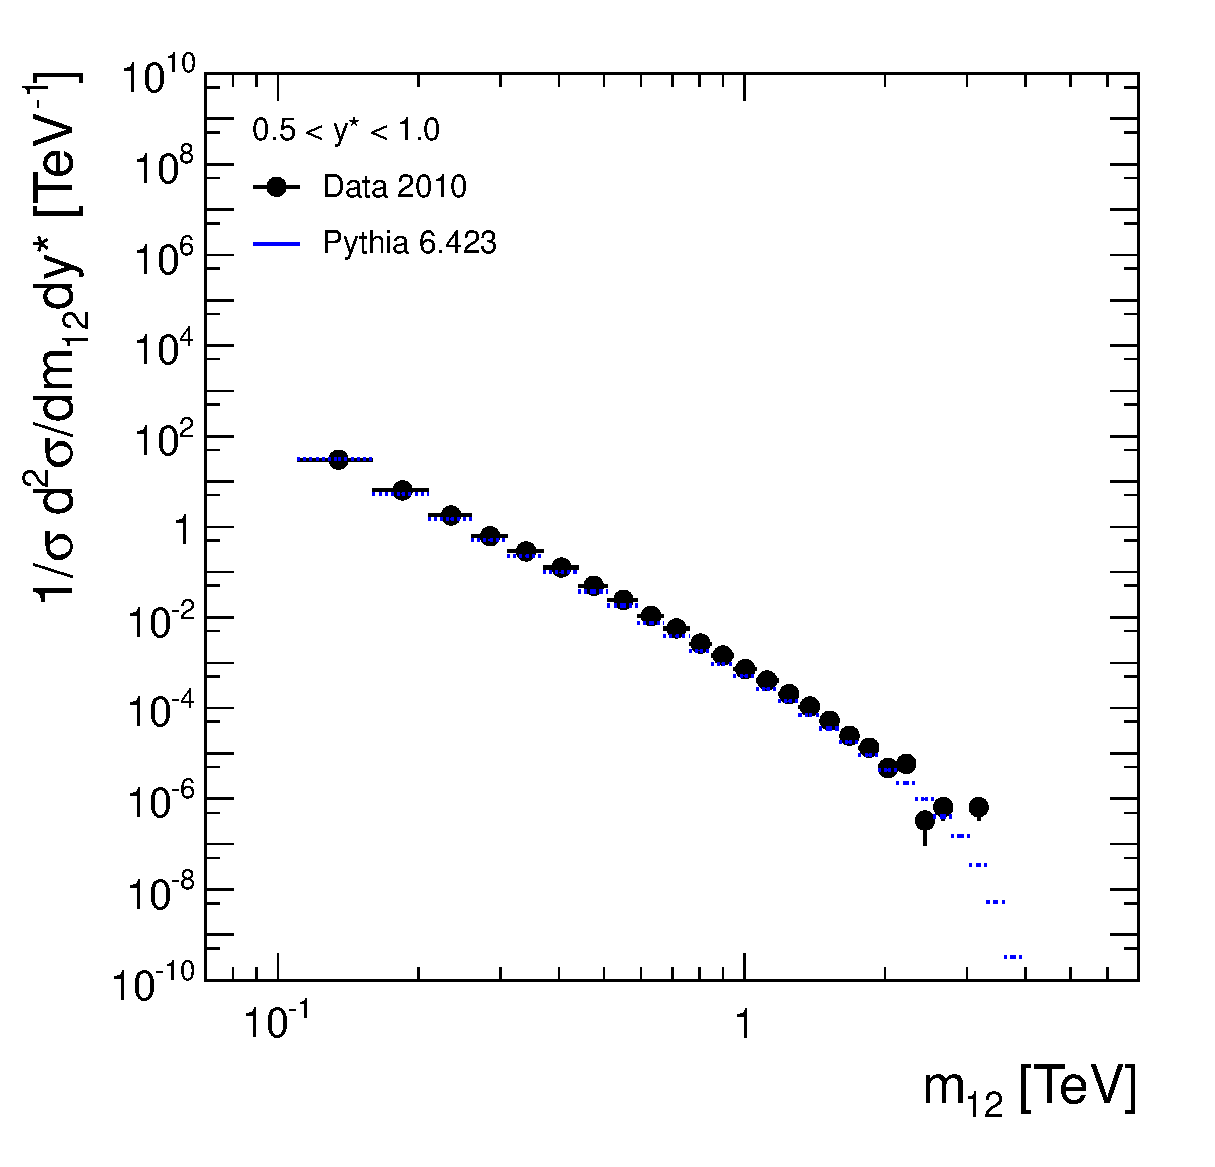
\includegraphics[width=\smallfigwidth]{chapters/dijets/Control.InclusiveDijets.AntiKt4.yStar0.5_1.eps}
    \label{fig:dijets:control_akt4_05_1}}
  \quad
  \subfloat[Data to \MC comparison for \akt $R=0.6$, in the region $2.0 \leq \yStar < 2.5$]{
    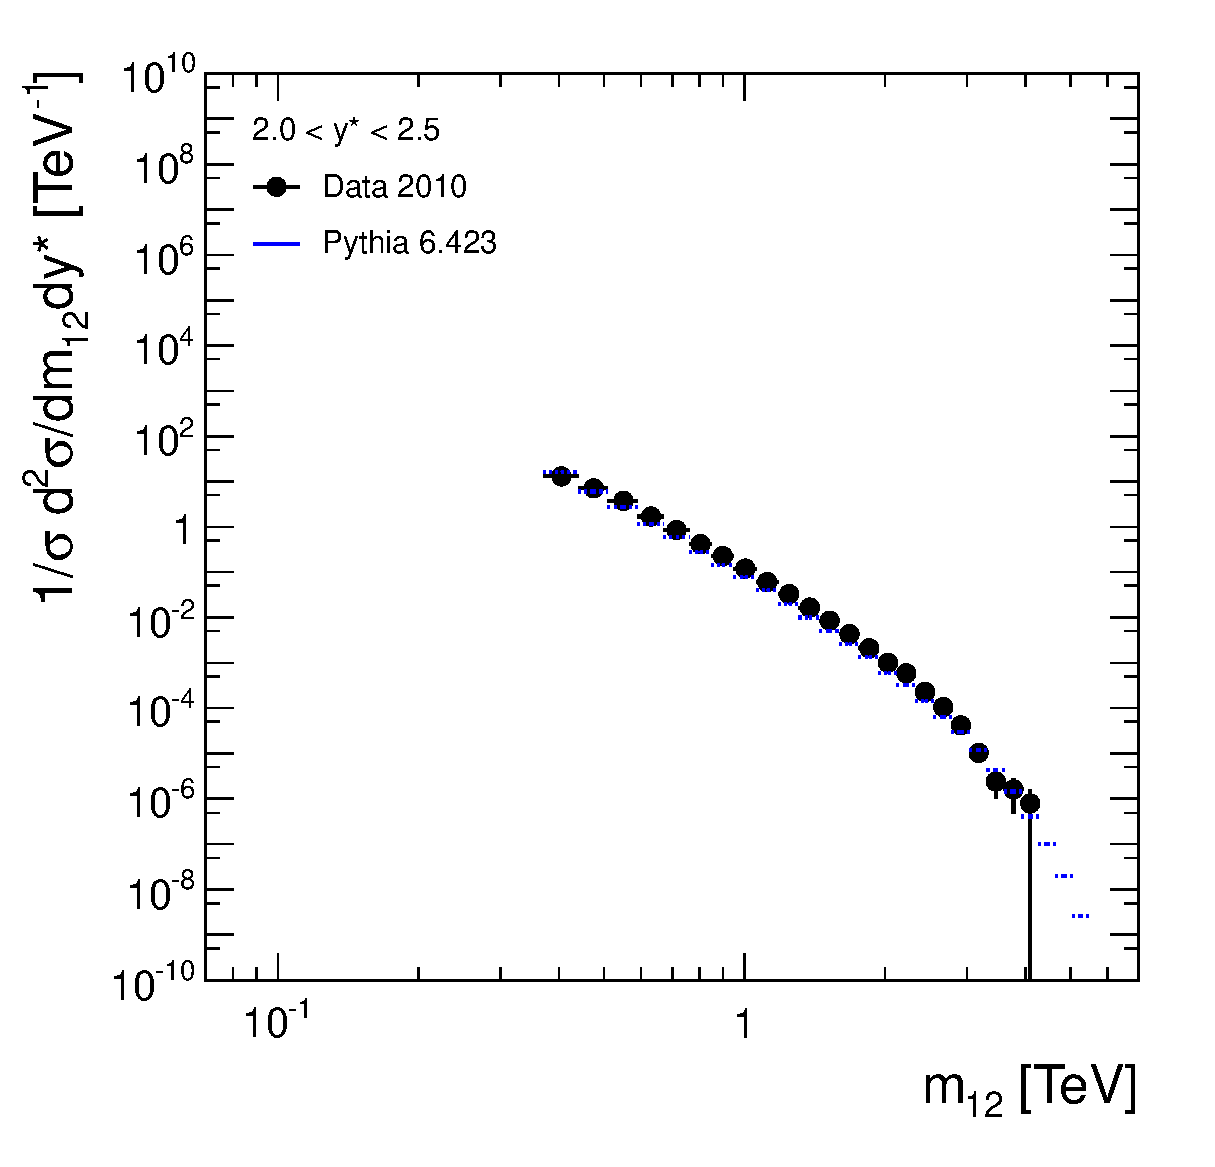
\includegraphics[width=\smallfigwidth]{chapters/dijets/Control.InclusiveDijets.AntiKt6.yStar2_2.5.eps}
    \label{fig:dijets:control_akt6_2_25}}
  \caption{Control distributions, used to demonstrate the level of agreement between data and \MC. Data is shown in black, with \Pythia in blue. \protect\subref{fig:dijets:control_akt4_05_1} shows the comparison for \akt $R=0.4$ jets in the region $0.5 \leq \yStar < 1.0$, while \protect\subref{fig:dijets:control_akt6_2_25} shows the comparison for \akt $R=0.6$ jets in the region $2.0 \leq \yStar < 2.5$.}
  \label{fig:dijets:data_mc_control_distributions}
\end{figure}

\section{Systematic Uncertainties}
The systematic uncertainties for the \dijet \xs measurements are calculated,
propagated and combined as described in \SectionRef{sec:forward-inclusive:systematics}.
The jet energy scale uncertainty is again the largest single contributor to the
overall uncertainty, dominating the other contributions, particularly in the
high mass region when the \xs is steeply falling.

\section{Theoretical Predictions}
Measured \dijet \xs{s} are compared to both NLO \pQCD predictions,
with corrections for non-perturbative effects, and to NLO \MC. The NLO
\pQCD predictions are produced using \NLOjetpp 4.1.2~\cite{Nagy:2003:NLOjet}
with the CT10~\cite{Lai:2010:LHAPDF_CT10} NLO PDFs while NLO \MC predictions
come from \Powheg, interfaced with both \Pythia and \Herwig. Uncertainties are
determined as outlined in \SectionRef{sec:forward-inclusive:theory_predictions}.

\section{Leading \Dijet \Xs{s}}
The \dijet double-differential \xs is measured as a function of the \dijet
invariant mass for nine bins of the variable \yStar, defined as
half the absolute value of the rapidity difference of the two leading jets, ranging
from 0 to 4.4. The results are shown in \FiguresRef{fig:dijets:InclusiveCrossSectionAKT4}{fig:dijets:InclusiveCrossSectionAKT6} for \akt jets with $R=0.4$
and $R=0.6$, respectively. The \xs falls rapidly with mass, and extends up to \dijet
masses of nearly \unit{5}{\TeV}.

\begin{figure}
  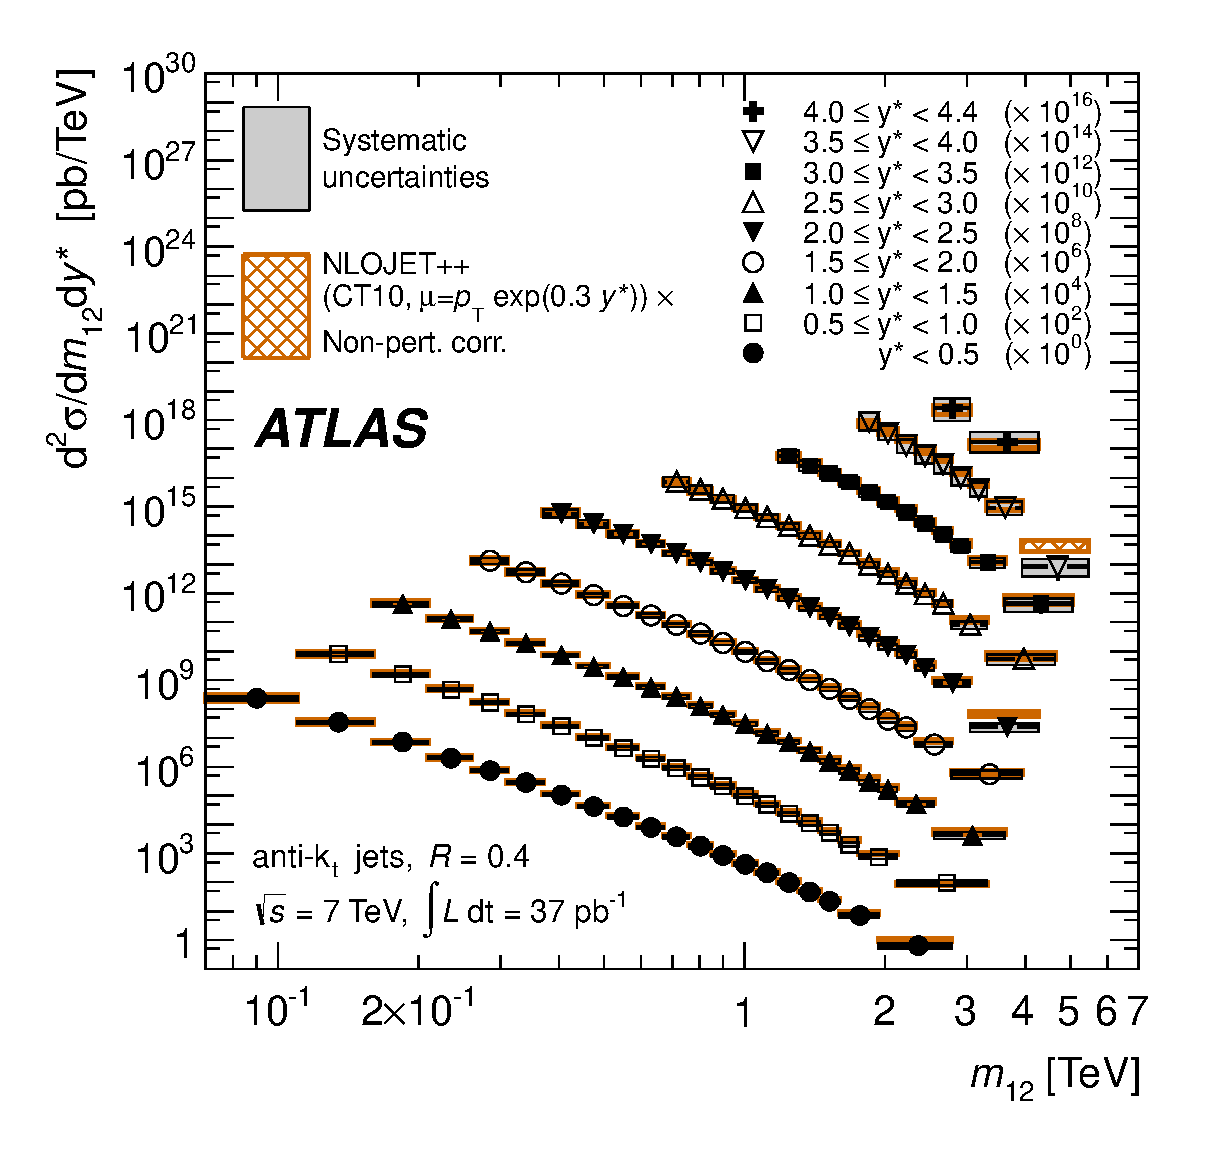
\includegraphics[width=\largefigwidth]{chapters/dijets/DijetMassYStarNLO_04.eps}
  \caption{\Dijet double-differential \xs as a function of \dijet mass, binned
     in half the rapidity separation between the two leading jets, $\yStar = |y_1 - y_2|/2$,
     for jets identified using the \akt algorithm with $R=0.4$. For convenience,
     the \xs{s} are multiplied by the factors indicated in the legend. The
     data are compared to NLO \pQCD calculations from \NLOjetpp, using the CT10
     PDF set and to which non-perturbative corrections have been applied. The error
     bars, which are usually smaller than the symbols, indicate the statistical
     uncertainty on the measurement. The dark-shaded band indicates the quadratic
     sum of the experimental systematic uncertainties, which are dominated by
     the jet energy scale uncertainty. There is an additional overall uncertainty
     of 3.4\% due to the luminosity measurement that is not shown. The theory uncertainty,
     shown as the light cross-hatched band, is the quadratic sum of uncertainties
     from the choice of the renormalisation and factorisation scales, PDFs, $\alphaS(M_Z)$,
     and the modelling of non-perturbative effects, as described in the text.}
  \label{fig:dijets:InclusiveCrossSectionAKT4}
\end{figure}


\begin{figure}
  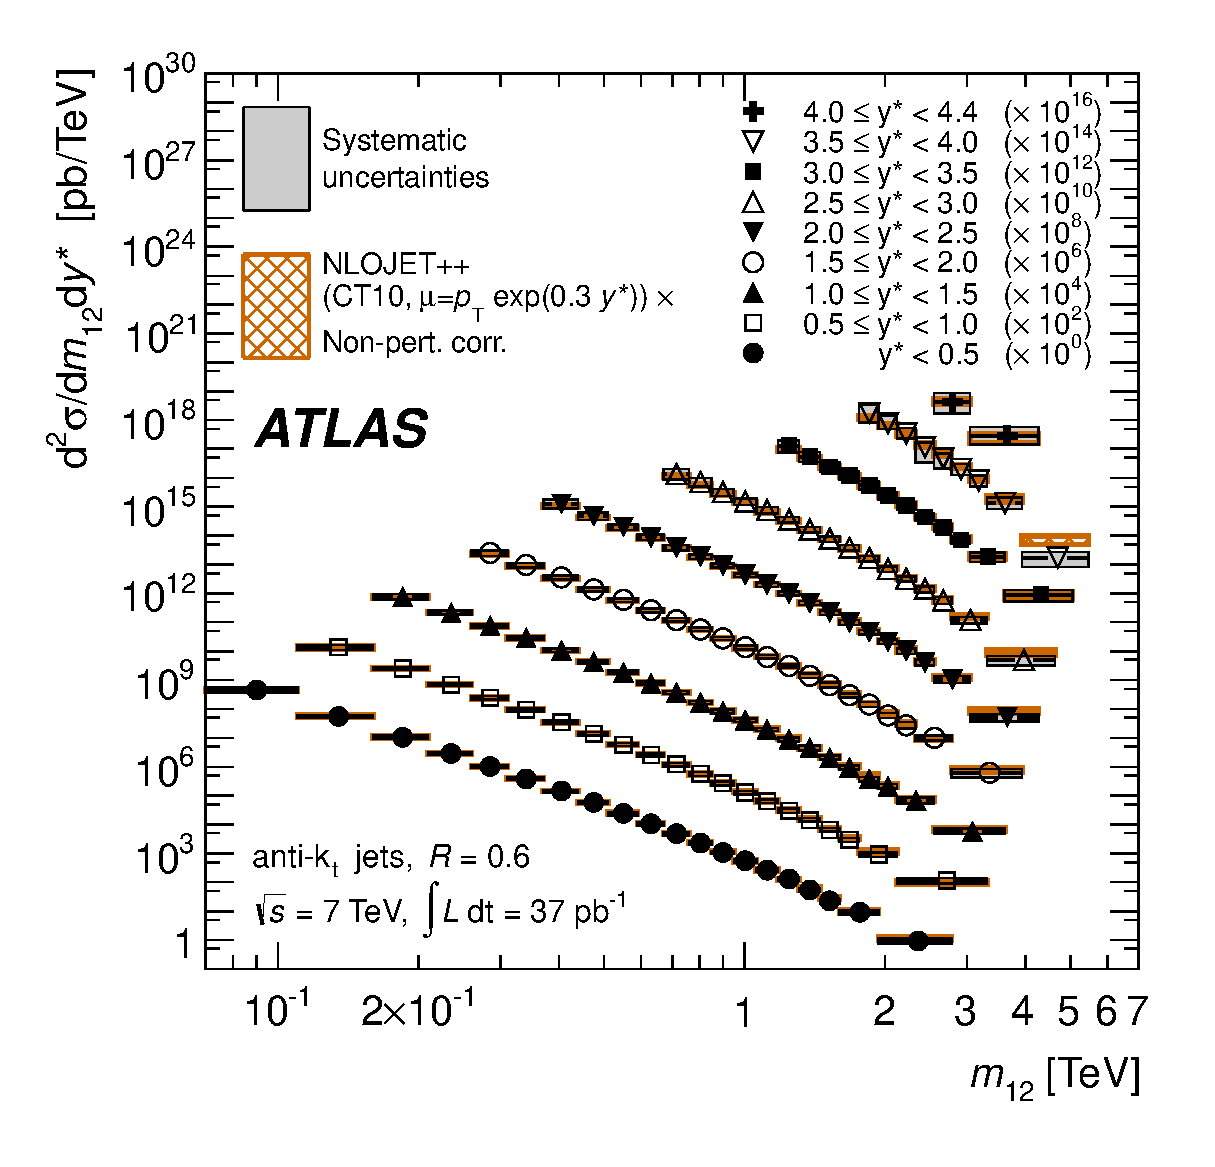
\includegraphics[width=\largefigwidth]{chapters/dijets/DijetMassYStarNLO_06.eps}
  \caption{\Dijet double-differential \xs as a function of \dijet mass, binned
     in half the rapidity separation between the two leading jets, $\yStar = |y_1 - y_2|/2$,
     for jets identified using the \akt algorithm with $R=0.6$. For convenience,
     the \xs{s} are multiplied by the factors indicated in the legend. The
     data are compared to NLO \pQCD calculations from \NLOjetpp, using the CT10
     PDF set and to which non-perturbative corrections have been applied. The systematic
     uncertainties are calculated as described in \FigureRef{fig:dijets:InclusiveCrossSectionAKT4}.}
  \label{fig:dijets:InclusiveCrossSectionAKT6}
\end{figure}

The comparison of the data with the \Powheg prediction, using the CT10 PDF set,
is shown in different \yStar regions in \FiguresRef{fig:dijets:PowhegRatio_akt4_central}{fig:dijets:PowhegRatio_akt4_forward}
for \akt jets with $R=0.4$ and in \FiguresRef{fig:dijets:PowhegRatio_akt6_central}{fig:dijets:PowhegRatio_akt6_forward}
for \akt jets with $R=0.6$. Here the data, \Powheg predictions interfaced with
\Pythia (AUET2B and \Perugia~2010 tunes) and \Herwig (AUET2 tune) and fixed order
\Powheg with non-perturbative corrections are all compared. The ratio of each of
these with respect to the NLO pQCD prediction (CT10 PDF set) baseline is shown.

As in the inclusive jets case, the \Powheg prediction agrees better with data
after being interfaced with \Pythia than with \Herwig. Since the same matrix
element, which agrees with the \NLOjetpp prediction, is used in both cases, this
provides further evidence that the \Pythia parton shower approach more
accurately reproduces the data than the angle-ordered parton shower used by
\Herwig. The \Perugia tune of \Pythia also performs badly, but this is a deliberately
extreme tune, which is not expected to agree well with the data. In general, the
\Herwig tunes used for these comparisons are perhaps not correctly optimised for
\LHC data - additional tunes may provide improved agreement in future.

%\begin{figure}[htbp]
%  \subfloat[\Akt $R=0.4$, small \yStar]{
%    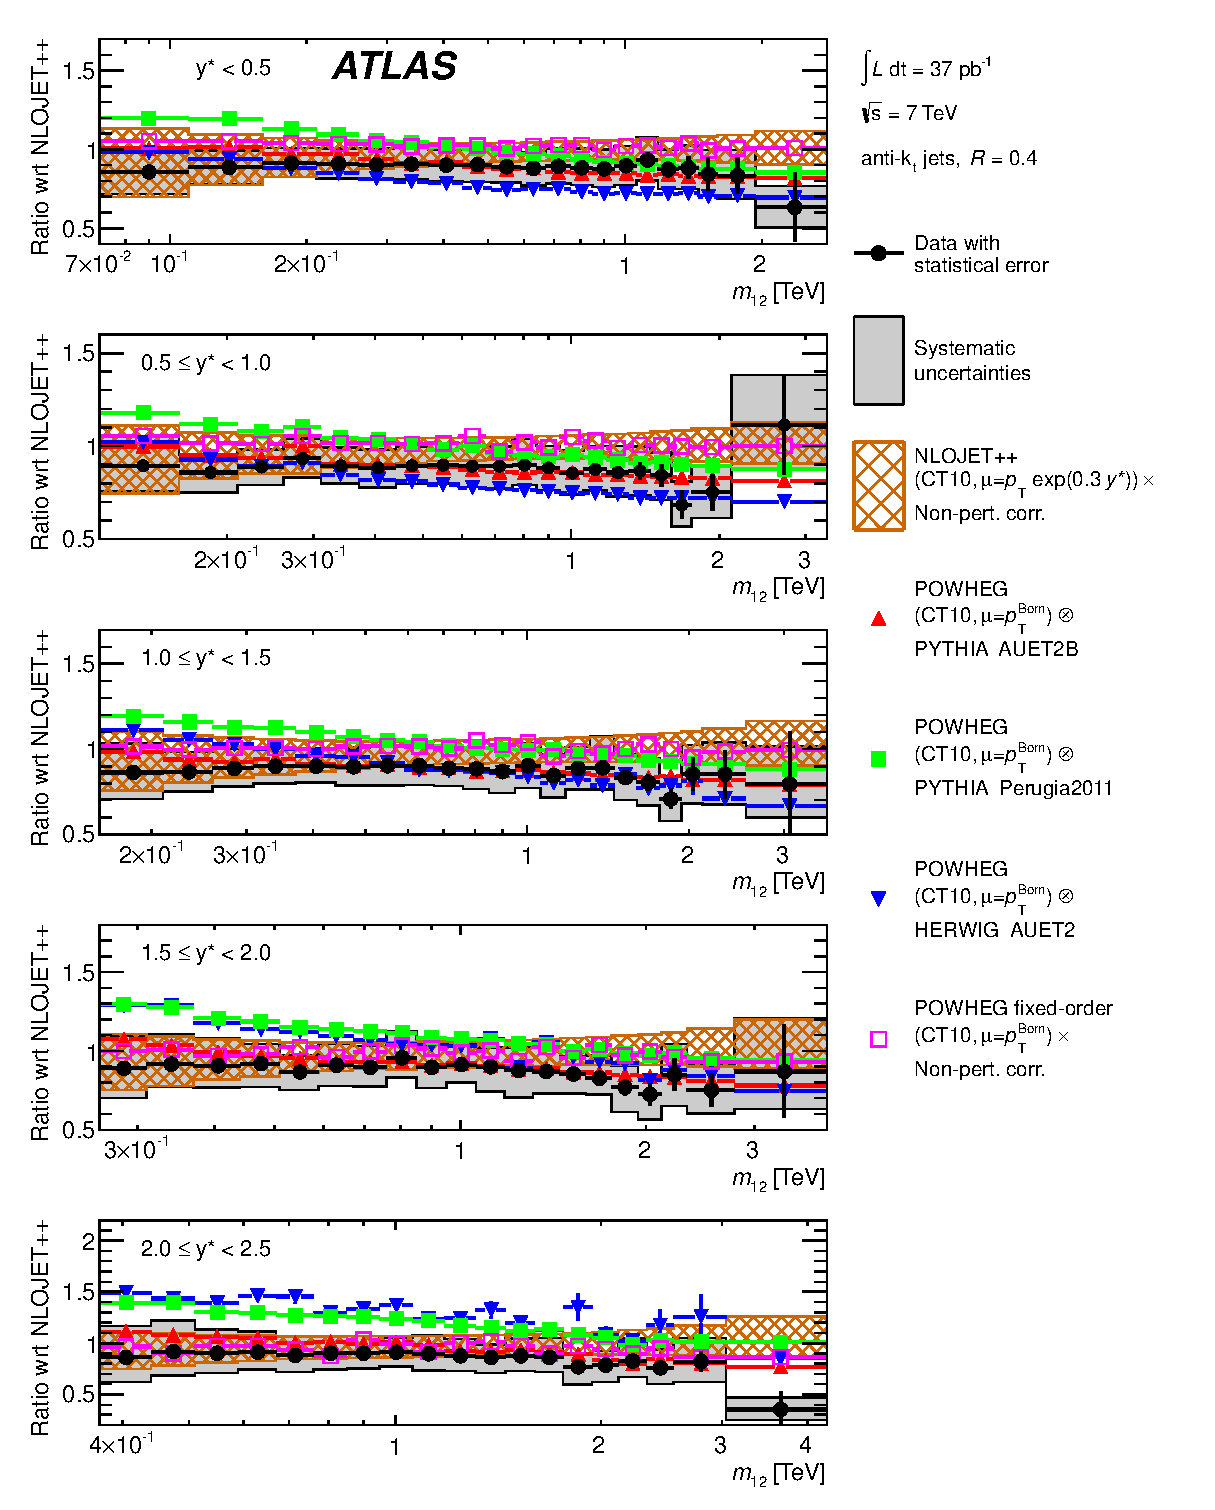
\includegraphics[width=\smallfigwidth]{chapters/dijets/DijetMassYStarRatioFinal04_central.eps}
%    \label{fig:dijets:PowhegRatioSmallYStar_akt4}}
%  \quad
%  \subfloat[\Akt $R=0.6$, small \yStar]{
%    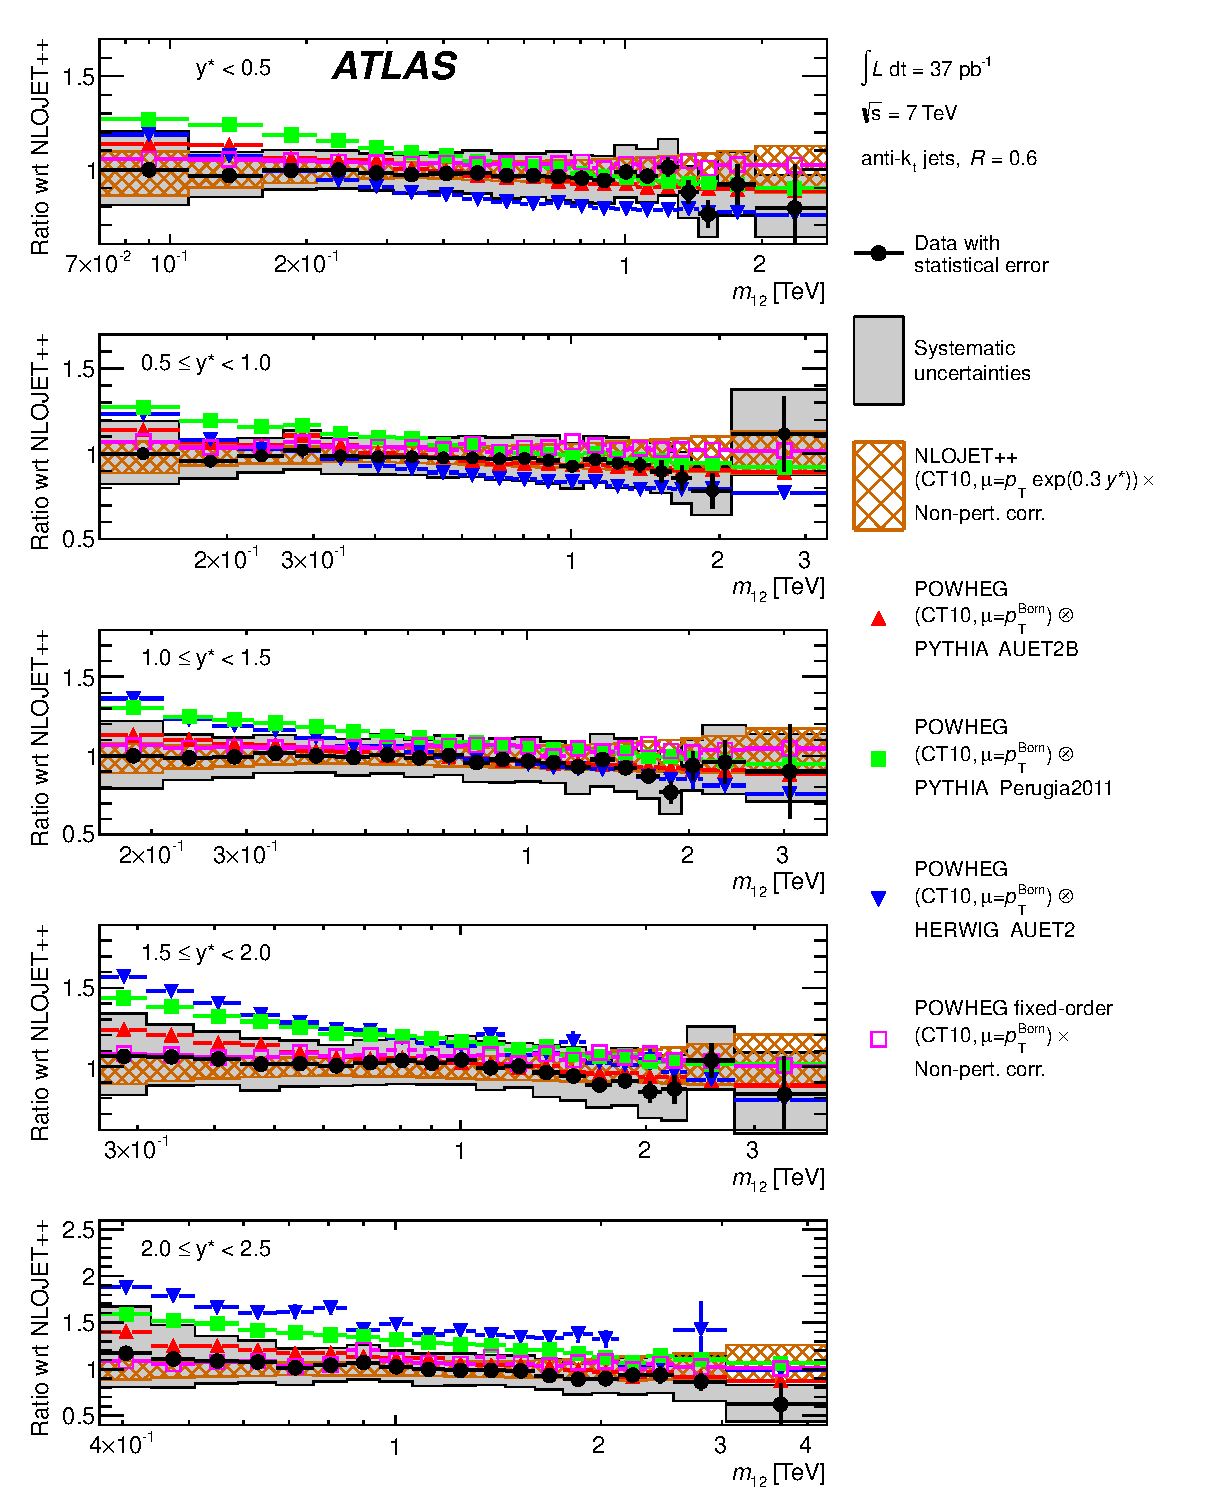
\includegraphics[width=\smallfigwidth]{chapters/dijets/DijetMassYStarRatioFinal06_central.eps}
%    \label{fig:dijets:PowhegRatioSmallYStar_akt6}}
%  \caption{Ratios of inclusive \dijet double-differential \xs to the theoretical
%           prediction obtained using \NLOjetpp with the CT10 PDF set. The ratios
%           are shown as a function of \dijet mass, binned in half the rapidity separation
%           between the two leading jets, $\yStar = |y_1 - y_2|/2$, for $0.0 \leq \yStar < 2.5$.
%           Jets are identified using the \akt algorithm with $R=0.4$ (left) and
%           $R=0.6$ (right). The ratios of \Powheg predictions, interfaced with either
%           \Pythia or \Herwig, to the \NLOjetpp predictions, corrected for non-perturbative
%           effects, are shown and can be compared to the corresponding ratios for
%           data. \Powheg ME calculations using the CT10 PDF set are also shown.
%           The total systematic uncertainties on the theory and the measurement
%           are indicated. Only the statistical uncertainty on the \Powheg predictions
%           is shown. The experimental uncertainties are calculated as described
%           in \FigureRef{fig:dijets:InclusiveCrossSectionAKT4}.}
%  \label{fig:dijets:PowhegRatio_A}
%\end{figure}

\begin{figure}
  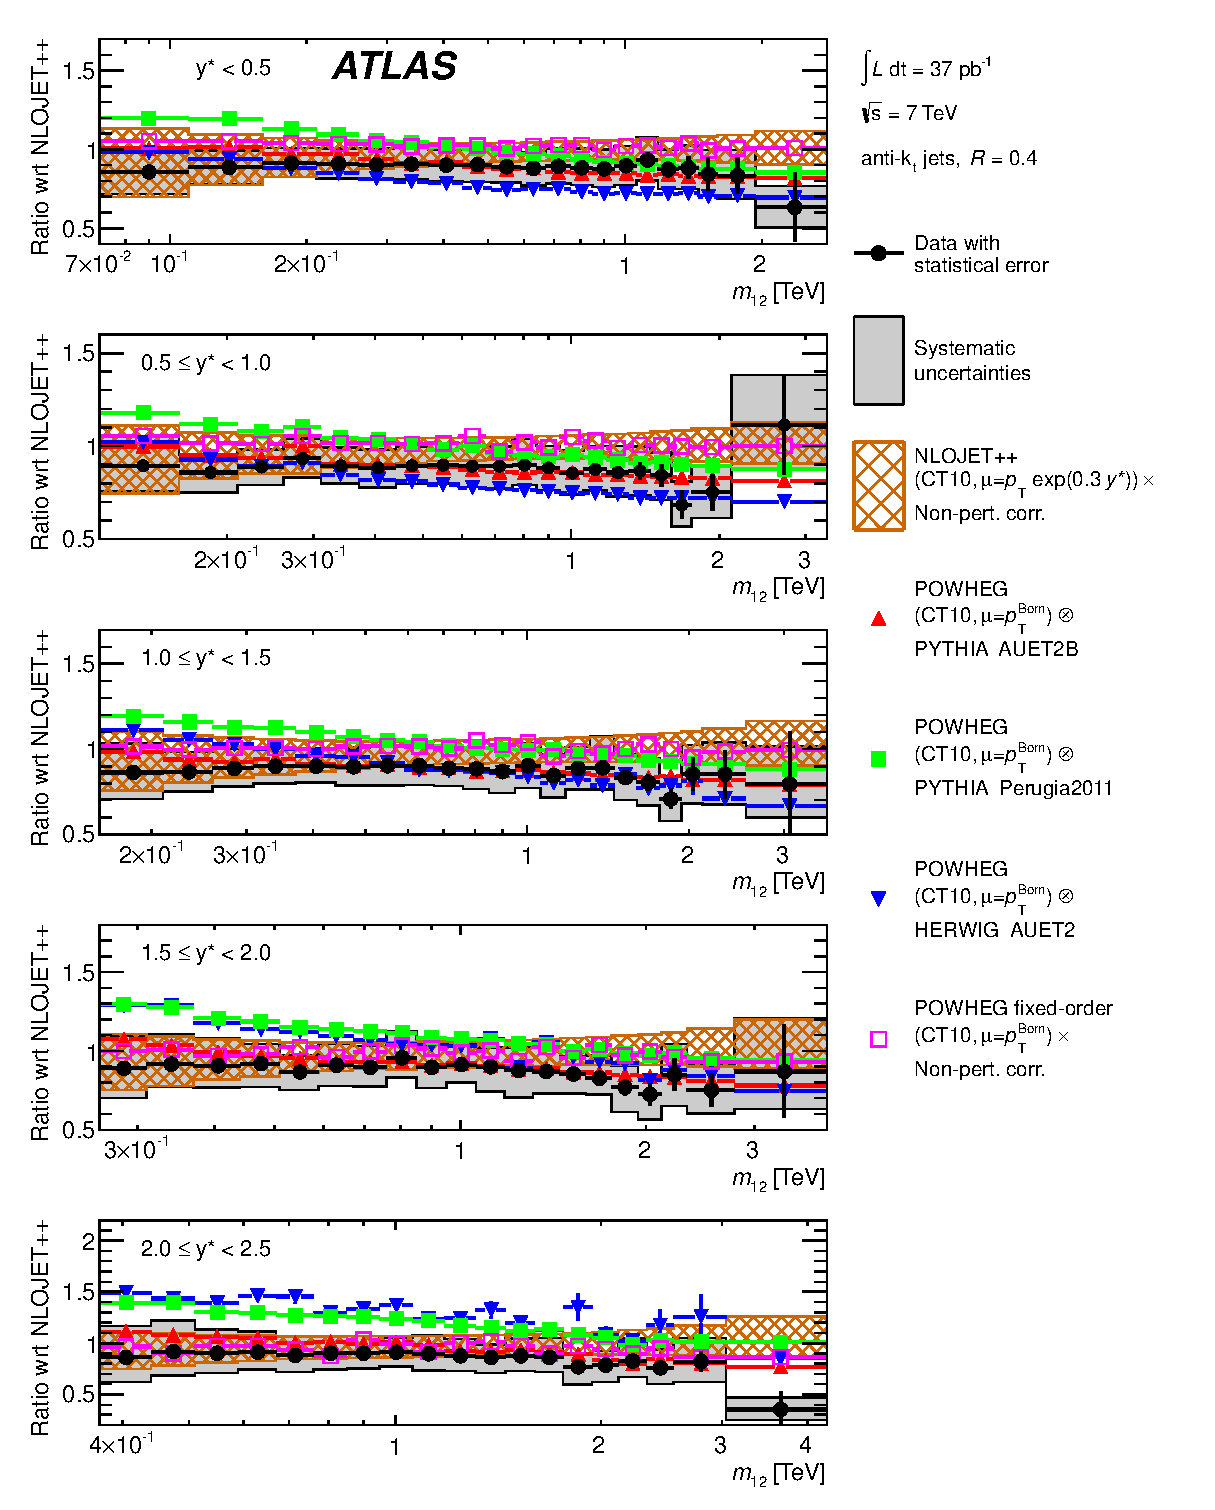
\includegraphics[width=\largefigwidth]{chapters/dijets/DijetMassYStarRatioFinal04_central.eps}
  \caption{Ratios of inclusive \dijet double-differential \xs to the theoretical
     prediction obtained using \NLOjetpp with the CT10 PDF set. The ratios
     are shown as a function of \dijet mass, binned in half the rapidity separation
     between the two leading jets, $\yStar = |y_1 - y_2|/2$, for $0.0 \leq \yStar < 2.5$.
     Jets are identified using the \akt algorithm with $R=0.4$. The plot shows the
     ratios of \Powheg predictions, interfaced with either \Pythia (AUET2B tune), \Pythia
     (\Perugia 2011 tune) or \Herwig, to the \NLOjetpp predictions, after these have
     been corrected for non-perturbative effects. The corresponding ratios for data
     are also shown for comparison. Additionally, \Powheg matrix-element calculations,
     also using the CT10 PDF set are shown. The total systematic uncertainties on
     the theory and the measurement are indicated. Only the statistical uncertainty
     on the \Powheg predictions is shown. The experimental uncertainties are calculated
     as described in \FigureRef{fig:dijets:InclusiveCrossSectionAKT4}.}
  \label{fig:dijets:PowhegRatio_akt4_central}
\end{figure}

\begin{figure}
  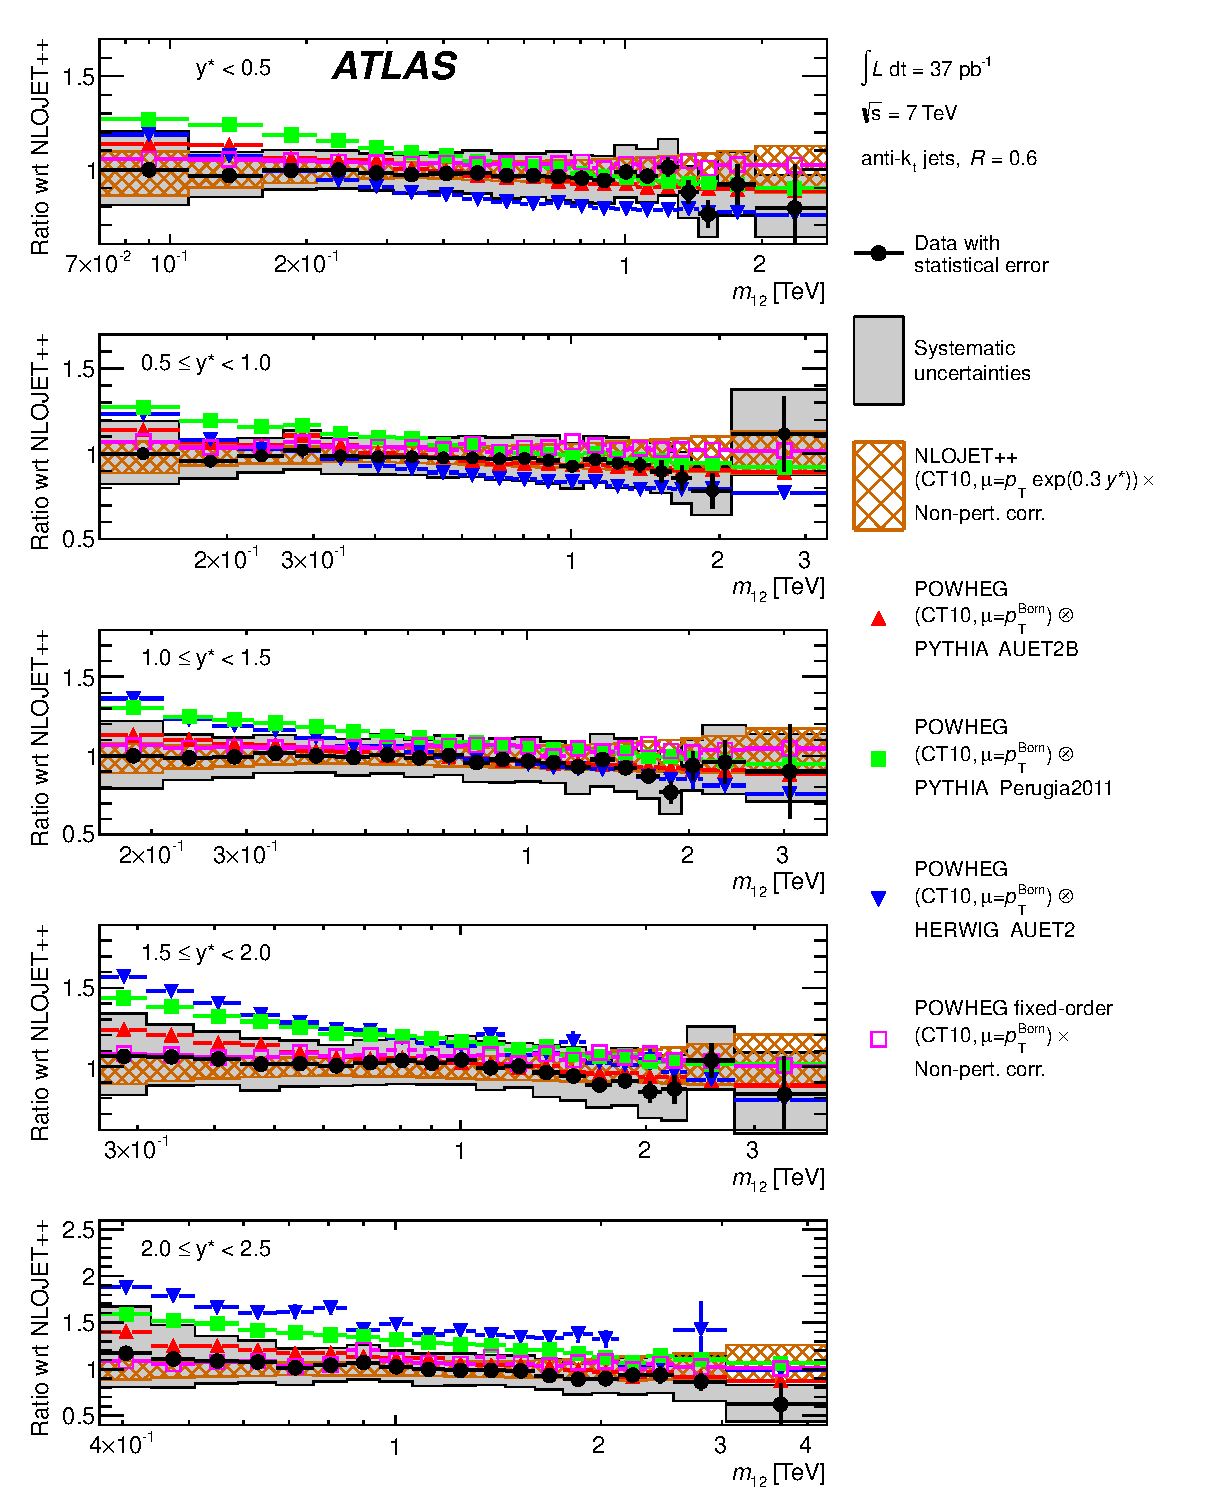
\includegraphics[width=\largefigwidth]{chapters/dijets/DijetMassYStarRatioFinal06_central.eps}
  \caption{Ratios of inclusive \dijet double-differential \xs to the theoretical
     prediction obtained using \NLOjetpp with the CT10 PDF set. The ratios
     are shown as a function of \dijet mass, binned in half the rapidity separation
     between the two leading jets, $\yStar = |y_1 - y_2|/2$, for $0.0 \leq \yStar < 2.5$.
     Jets are identified using the \akt algorithm with $R=0.6$. The plot shows the
     ratios of \Powheg predictions, interfaced with either \Pythia (AUET2B tune), \Pythia
     (\Perugia 2011 tune) or \Herwig, to the \NLOjetpp predictions, after these have
     been corrected for non-perturbative effects. The corresponding ratios for data
     are also shown for comparison. Additionally, \Powheg matrix-element calculations,
     also using the CT10 PDF set are shown. Uncertainties are as described in
     \FigureRef{fig:dijets:PowhegRatio_akt4_central}.}
  \label{fig:dijets:PowhegRatio_akt6_central}
\end{figure}

%\begin{figure}[htbp]
%  \subfloat[\Akt $R=0.4$, large \yStar]{
%    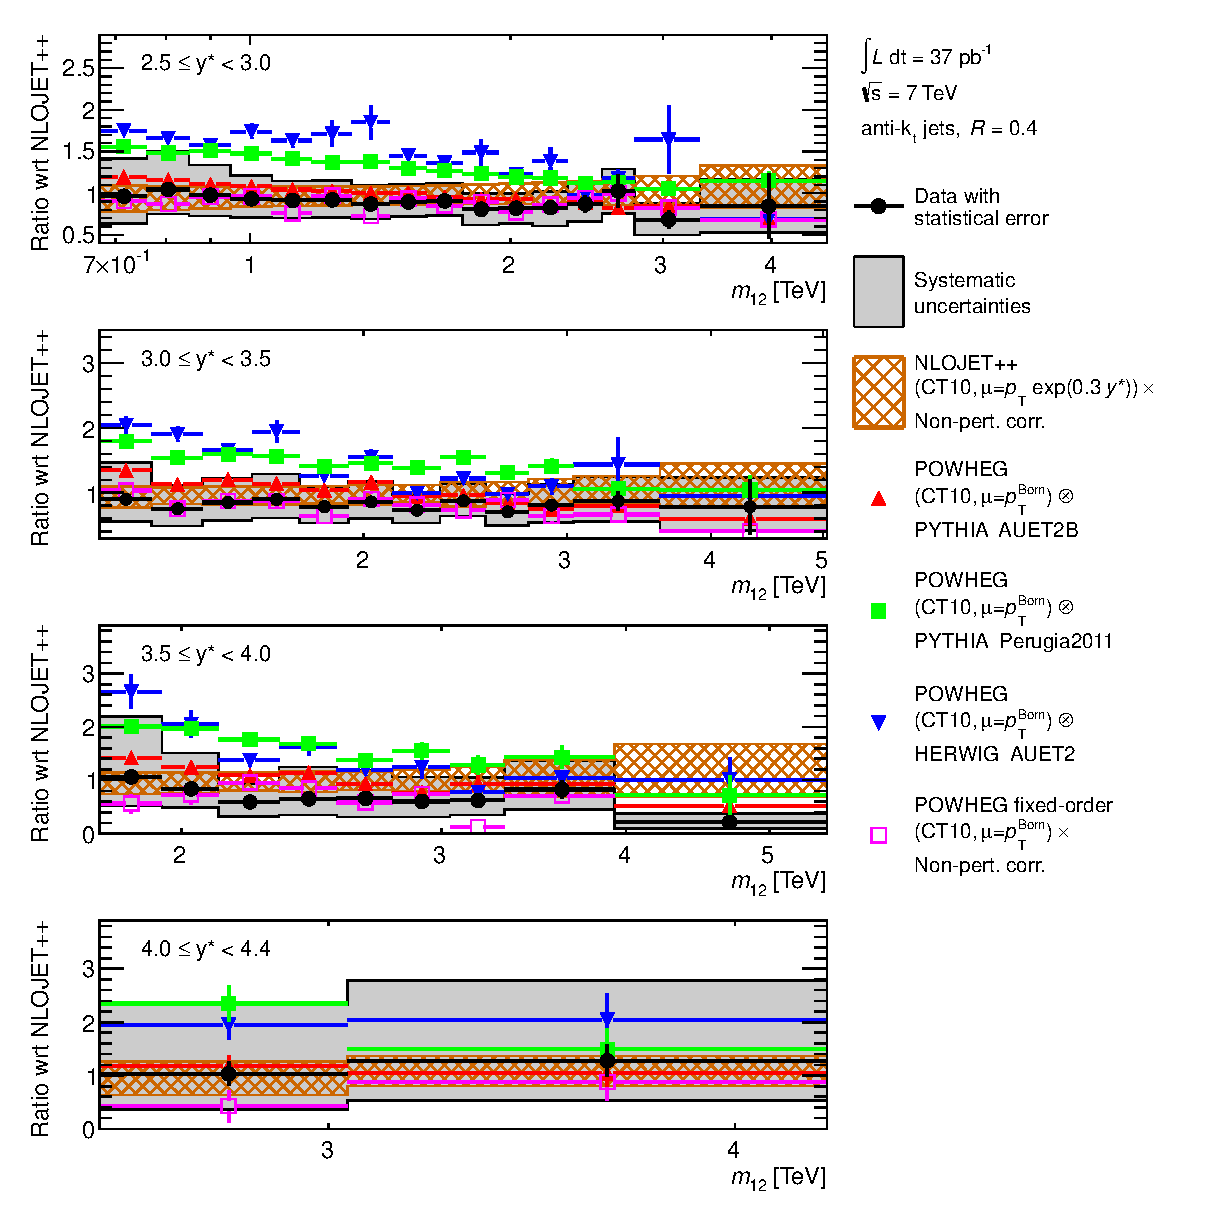
\includegraphics[width=\smallfigwidth]{chapters/dijets/DijetMassYStarRatioFinal04_forward.eps}
%    \label{fig:dijets:PowhegRatioLargeYStar_akt4}}
%  \quad
%  \subfloat[\Akt $R=0.6$, large \yStar]{
%    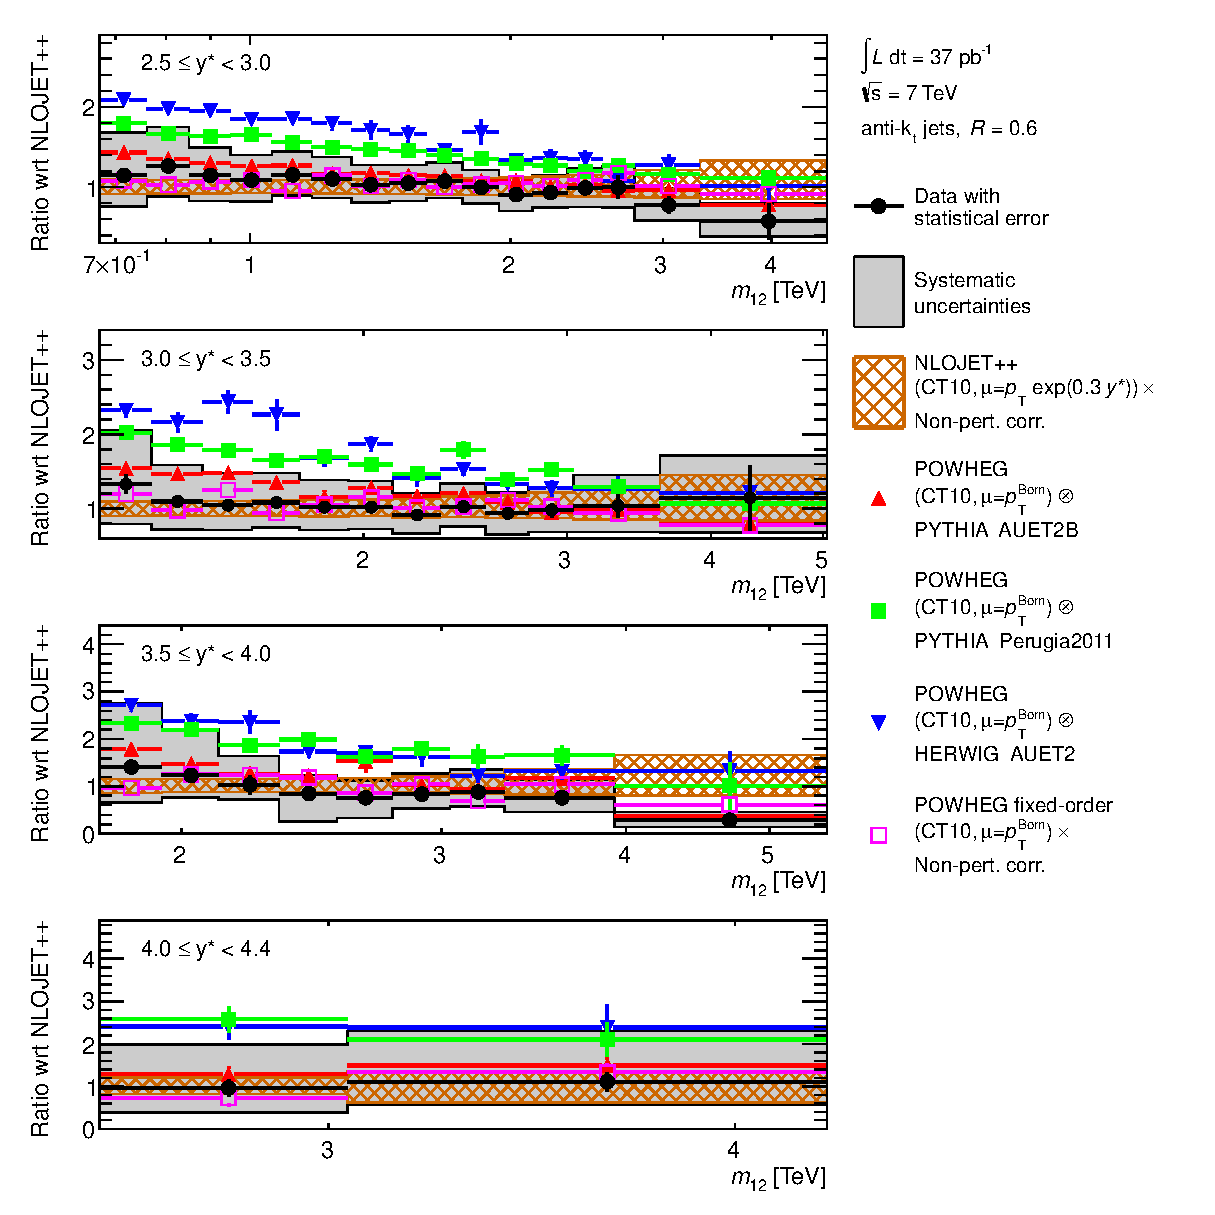
\includegraphics[width=\smallfigwidth]{chapters/dijets/DijetMassYStarRatioFinal06_forward.eps}
%    \label{fig:dijets:PowhegRatioLargeYStar_akt6}}
%  \caption{Ratios of inclusive \dijet double-differential \xs to the theoretical
%           prediction obtained using \NLOjetpp with the CT10 PDF set. The ratios
%           are shown as a function of \dijet mass, binned in half the rapidity separation
%           between the two leading jets, $\yStar = |y_1 - y_2|/2$, for $2.5 \leq \yStar < 4.4$.
%           Jets are identified using the \akt algorithm with $R=0.4$ (left) and
%           $R=0.6$ (right). The ratios of \Powheg predictions, interfaced with either
%           \Pythia or \Herwig, to the \NLOjetpp predictions, corrected for non-perturbative
%           effects, are shown and can be compared to the corresponding ratios for
%           data. \Powheg ME calculations using the CT10 PDF set are also shown.
%           Uncertainties are as described in \FigureRef{fig:dijets:PowhegRatio_A}.}
%  \label{fig:dijets:PowhegRatio_B}
%\end{figure}

\begin{figure}
  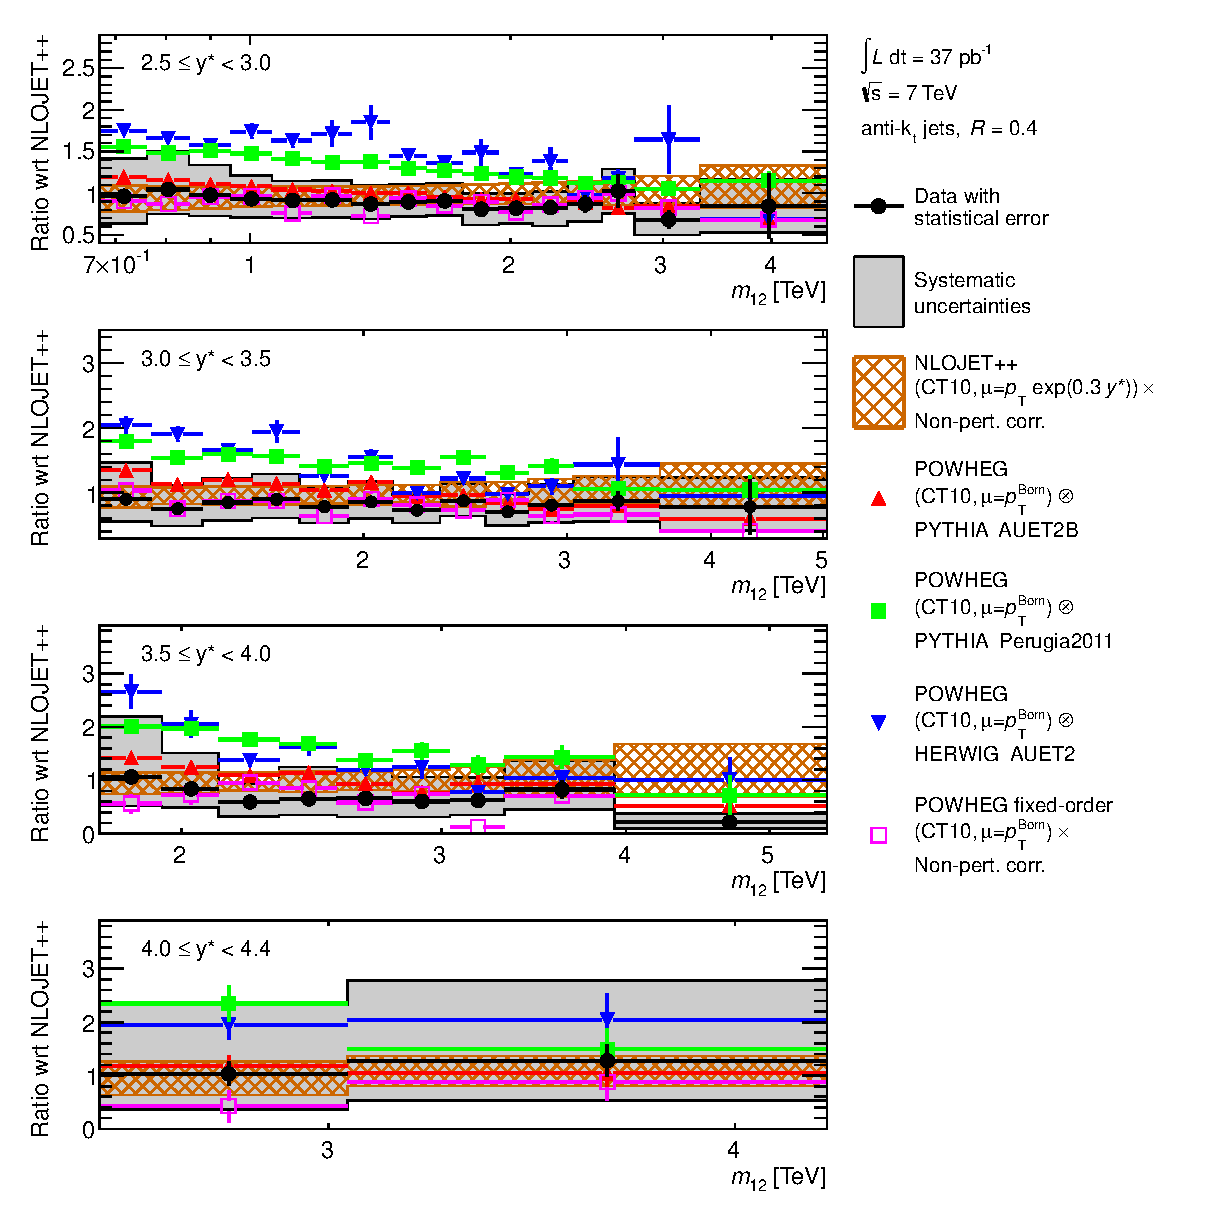
\includegraphics[width=\largefigwidth]{chapters/dijets/DijetMassYStarRatioFinal04_forward.eps}
  \caption{Ratios of inclusive \dijet double-differential \xs to the theoretical
     prediction obtained using \NLOjetpp with the CT10 PDF set. The ratios
     are shown as a function of \dijet mass, binned in half the rapidity separation
     between the two leading jets, $\yStar = |y_1 - y_2|/2$, for $2.5 \leq \yStar < 4.4$.
     Jets are identified using the \akt algorithm with $R=0.4$. The plot shows the
     ratios of \Powheg predictions, interfaced with either \Pythia (AUET2B tune), \Pythia
     (\Perugia 2011 tune) or \Herwig, to the \NLOjetpp predictions, after these have
     been corrected for non-perturbative effects. The corresponding ratios for data
     are also shown for comparison. Additionally, \Powheg matrix-element calculations,
     also using the CT10 PDF set are shown. Uncertainties are as described in
     \FigureRef{fig:dijets:PowhegRatio_akt4_central}.}
  \label{fig:dijets:PowhegRatio_akt4_forward}
\end{figure}

\begin{figure}
  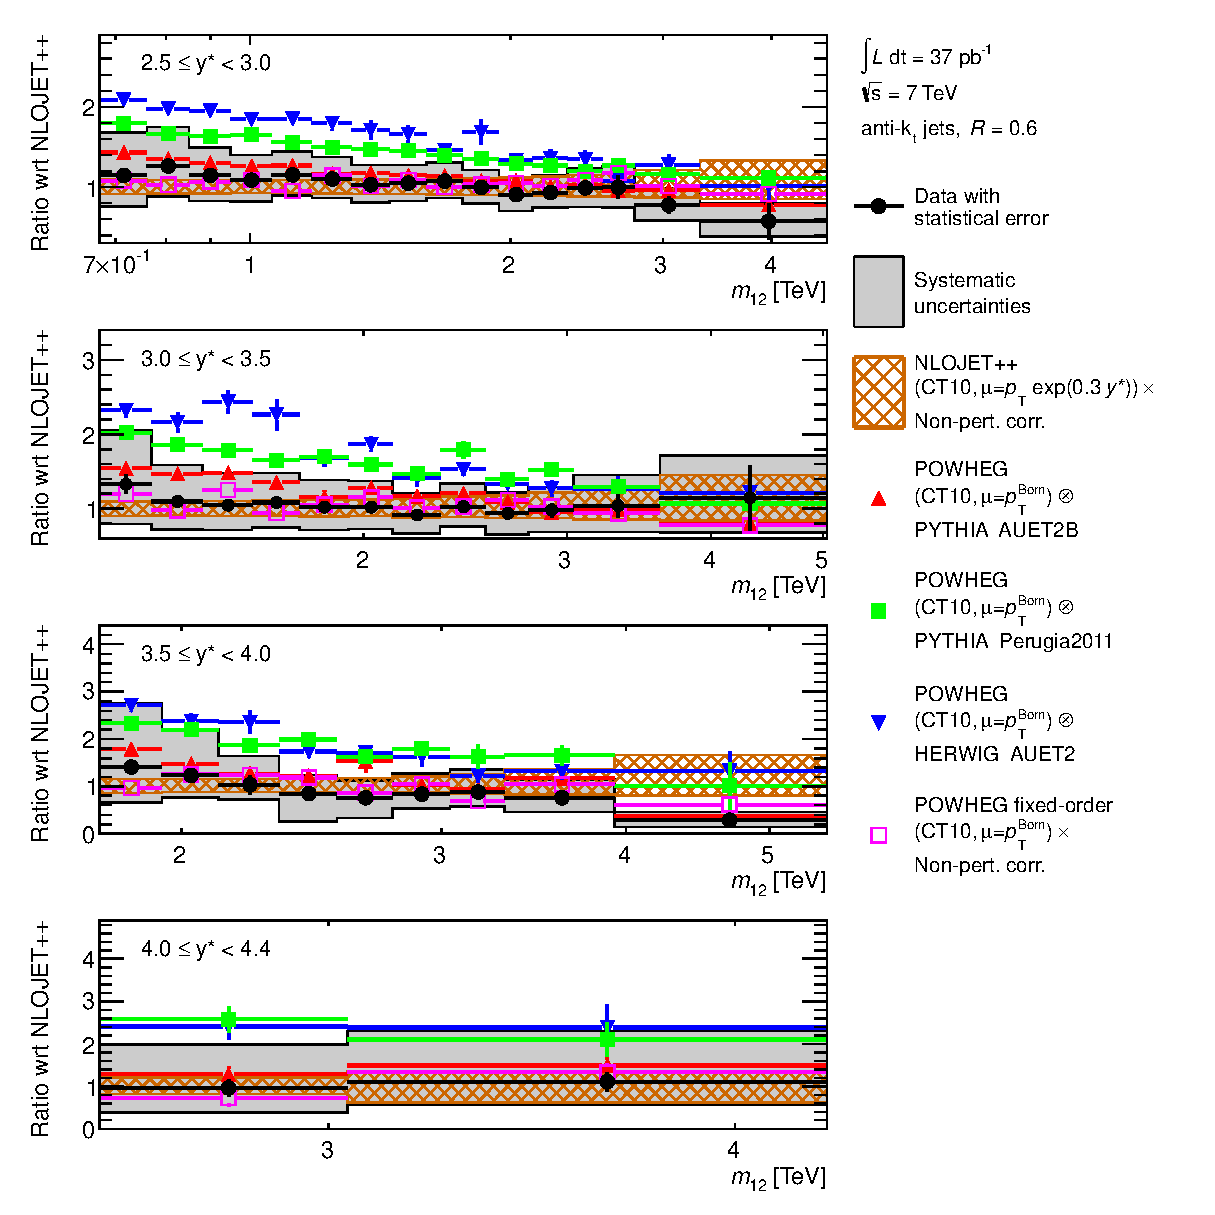
\includegraphics[width=\largefigwidth]{chapters/dijets/DijetMassYStarRatioFinal06_forward.eps}
  \caption{Ratios of inclusive \dijet double-differential \xs to the theoretical
     prediction obtained using \NLOjetpp with the CT10 PDF set. The ratios
     are shown as a function of \dijet mass, binned in half the rapidity separation
     between the two leading jets, $\yStar = |y_1 - y_2|/2$, for $2.5 \leq \yStar < 4.4$.
     Jets are identified using the \akt algorithm with $R=0.6$. The plot shows the
     ratios of \Powheg predictions, interfaced with either \Pythia (AUET2B tune), \Pythia
     (\Perugia 2011 tune) or \Herwig, to the \NLOjetpp predictions, after these have
     been corrected for non-perturbative effects. The corresponding ratios for data
     are also shown for comparison. Additionally, \Powheg matrix-element calculations,
     also using the CT10 PDF set are shown. Uncertainties are as described in
     \FigureRef{fig:dijets:PowhegRatio_akt4_central}.}
  \label{fig:dijets:PowhegRatio_akt6_forward}
\end{figure}



\section{Summary}
Through the use of a complicated trigger strategy involving the combination of
multiple triggers from different trigger systems, it has been possible to
measure \dijet \xs{s} across a wide range of mass and rapidity separations,
reaching higher in \yStar than has previously been possible.

Jets are reconstructed using the \akt algorithm with $R=0.4$ and $R=0.6$ in
order to probe the relative effects of the parton shower, hadronisation and
underlying event. Overall, the agreement of the NLO perturbative QCD predictions
with the measurements extends over seven orders of magnitude in \xs: presenting an impressive validation of \QCD
over a range of phase space.

As discussed in \SectionRef{sec:forward-inclusive:conclusions}, the experimental
uncertainties are comparable to the theoretical uncertainties in some regions of
phase space, providing sensitivity to different predictions. Differences between
the NLO pQCD calculation and NLO \MC predictions are, however, of the same order
as the NLO scale variation and are hence inconclusive. This work has been
published, together with the inclusive jet \xs{s} in the European Physical
Journal C~\cite{EPJC:2011:ATLASInclusiveJets} with an updated version submitted
to Physical Review D~\cite{CERN-PH-EP-2011-192}.
